% \iffalse meta-comment
%
% Copyright (C) 2022 by Skippi \url{https://github.com/Skipp1/fortex}
% ---------------------------------------------------------------------------
% This work may be distributed and/or modified under the
% conditions of the LaTeX Project Public License, either version 1.3
% of this license or (at your option) any later version.
% The latest version of this license is in
%   http://www.latex-project.org/lppl.txt
% and version 1.3 or later is part of all distributions of LaTeX
% version 2005/12/01 or later.
%
% This work has the LPPL maintenance status `maintained'.
%
% The Current Maintainer of this work is Skippi.
%
% This work consists of the files fortex.dtx and fortex.ins
% and the derived filebase fortex.sty.
%
%
%<*driver>
\documentclass[cm-default, a4paper]{l3doc}
\usepackage[T1, OT1]{fontenc}
\usepackage{expl3}
\usepackage[UKenglish]{babel}
\usepackage[dvipsnames]{xcolor}
\usepackage[scale=0.95, nottdefault]{sourcecodepro}
\usepackage{microtype}
\usepackage[skins, breakable]{tcolorbox}
\usepackage{tikz}
\usepackage{listings}
\usepackage{bookmark}
\usepackage[pass]{geometry}
\usetikzlibrary{decorations.pathmorphing}
\EnableCrossrefs
\lstset {
  , gobble=3
  , language=[LaTeX]TeX
  , basicstyle=\small\ttfamily
  , numbers=left
  , firstnumber=1
  , numberfirstline=true
  , tabsize=2
  , showstringspaces=false
  , commentstyle=\color[gray]{0.4}
  , stringstyle=\color{Rhodamine}
  , keywordstyle=\color{orange}
  , backgroundcolor = \color{lightgray!10}
}

\NewDocumentEnvironment{examplefile}{ O{} v m } {
  \def\ttdefault{SourceCodePro-TLF}
  \begin{tcolorbox}[{
    , title={#2} 
    , fonttitle=\large\fontfamily{cmtt}\selectfont
    , enhanced
    , attach boxed title to top left={yshift=-2mm}
    , pad at break = 1mm
    , underlay boxed title = { 
      \node[yshift=-10pt, xshift=-3pt] at (frame.north east) { \resizebox{30pt}{!}{\usebox{#3}} }; }
    , overlay first={
      \begin{scope}[decoration={zigzag,amplitude=0.5mm}]
        \path[fill=gray!10] decorate {([xshift=1.5pt]frame.south west) -- ([xshift=-1.5pt]frame.south east)} --++ (0,  0.5ex) -| cycle;
        \path[fill=white  ] decorate {([xshift=1.5pt]frame.south west) -- ([xshift=-1.5pt]frame.south east)} --++ (0, -0.5ex) -| cycle;
        \draw[thick, gray, decorate]  ([xshift=1.5pt]frame.south west) -- ([xshift=-1.5pt]frame.south east); 
      \end{scope}}
    , overlay last={
      \begin{scope}[decoration={zigzag,amplitude=0.5mm}]
        \path[fill=white  ] decorate {([xshift=1.5pt]frame.north west) -- ([xshift=-1.5pt]frame.north east)} --++ (0,  0.5ex) -| cycle;
        \path[fill=gray!10] decorate {([xshift=1.5pt]frame.north west) -- ([xshift=-1.5pt]frame.north east)} --++ (0, -0.5ex) -| cycle;
        \draw[thick, gray, decorate]  ([xshift=1.5pt]frame.north west) -- ([xshift=-1.5pt]frame.north east); 
      \end{scope}}
    , #1
  }]
} {
  \end{tcolorbox}
}

\ExplSyntaxOn
\cs_set_eq:NN \DescribeOption_aux:n \DescribeOption
\RenewDocumentCommand { \DescribeOption } { v m o } {
  \label { doc/function//#1 }
  \DescribeOption_aux:n { #1 } \textsf{ (~#2~) } \hfill \tl_if_novalue:nF { #3 } {Default:~\texttt{#3}}
  \newline \indent \use:n % gobble the stray space that appears?
}

\NewDocumentEnvironment { DescribeOptionIndent } { v m o } {
  \vspace{0.6\baselineskip}
  \noindent
  \begin{tabular*}{\textwidth}{@{}p{1.3cm}l@{\extracolsep{\fill}}r@{}}
  \texttt{#1} & \textsf { (~#2~) } &  \tl_if_novalue:nF { #3 } { Default:~\texttt { #3 } }
  \end{tabular*} 
  \list{}{
    \topsep=\parskip
    \leftmargin=\parindent
    \rightmargin=\parindent
  }\item
}{
  \endlist
}

\NewDocumentCommand { \optref } { m } { \hyperref [ doc/function//#1  ] { \texttt { #1 } } }
\NewDocumentCommand { \cbref  } { m } { \hyperref [ code:codeblock/#1 ] { \texttt { #1 } } }
\NewDocumentCommand { \csref  } { m } {
  \hyperref [ doc/function//#1  ] { \tn { #1 } }
}

% Make environment Environments linkable
\cs_set_eq:NN \environment_aux:n \environment
\RenewDocumentCommand{\environment}{v}{ 
  \label{doc/function//#1}
  \environment_aux:n {#1}
}

% Add hyperlinks to the env command
\cs_set_eq:NN \env_aux:n \env
\RenewDocumentCommand { \env } { v } {
 \hyperref [ doc/function//#1 ] { \env_aux:n { #1 } }
}

% Prevent overfull hboxes
\RenewDocumentEnvironment{syntax}{}{
  \ttfamily \small \hspace{\parindent}
  \begin{minipage}[t]{\linewidth-\parindent}
    \raggedright
    \obeyspaces
    \obeylines
}{
  \end{minipage}
  \vspace{\baselineskip}
}

% Try to avoid using cm-super.
% Also these should be fragile as they are used in \section{}, so we cannot use \NewDocumentCommand.
\def\lmold#1{{\fontencoding{T1}\fontfamily{lmr}\selectfont \oldstylenums{#1}}}
\def\textttbf#1{{\fontencoding{T1}\fontfamily{lmtt}\fontseries{b}\selectfont #1}}

\ExplSyntaxOff

% Only use when the index title is orphaned. 
% \setlength\IndexMin{100pt}

% File logo for C programming language 
\newsavebox\clogo
\sbox{\clogo}{
  
\begin{tikzpicture}[very thick]
    \draw[fill=CornflowerBlue!50] (0,0) -- (1-.3,0) -- (1,-.3)[rounded corners=1pt] -- (1, -1.3) -- (0, -1.3) -- cycle;
    \draw[rounded corners=1pt, fill=CornflowerBlue!25] (1-.3,0) -- (1-0.3,-.3)[rounded corners=0.2pt] -- (1, -.3) -- cycle ;
    \node at (0.49, -0.7) {\usefont{T1}{phv}{m}{n}\fontsize{16}{16}\selectfont C};
  \end{tikzpicture}
}

% File logo for Fortran90 programming language 
\newsavebox\flogo
\sbox{\flogo}{
  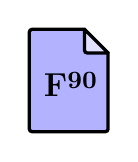
\begin{tikzpicture}[very thick]
    \draw[fill=blue!30] (0,0) -- (1-.3,0) -- (1,-.3)[rounded corners=1pt] -- (1, -1.3) -- (0, -1.3) -- cycle;
    \draw[rounded corners=1pt, fill=blue!12] (1-.3,0) -- (1-0.3,-.3)[rounded corners=0.2pt] -- (1, -.3) -- cycle ;
    \node at (0.52, -0.7) {\bfseries\large{F\small{\raisebox{2.7pt}{90}}}};
  \end{tikzpicture}
}

% File logo for Python programming language 
\newsavebox\pylogo
\sbox{\pylogo}{
  
\begin{tikzpicture}[very thick]
    \draw[fill=LimeGreen!35] (0,0) -- (1-.3,0) -- (1,-.3)[rounded corners=1pt] -- (1, -1.3) -- (0, -1.3) -- cycle;
    \draw[rounded corners=1pt, fill=LimeGreen!12] (1-.3,0) -- (1-0.3,-.3)[rounded corners=0.2pt] -- (1, -.3) -- cycle ;
    \node at (0.5, -0.7) {\usefont{T1}{iwona}{m}{n}\fontsize{15}{15}\selectfont py};
  \end{tikzpicture}
}

% File logo for TeX programming language 
\newsavebox\texlogo
\sbox{\texlogo}{
  
\begin{tikzpicture}[very thick]
    \draw[fill=Mulberry!30] (0,0) -- (1-.3,0) -- (1,-.3)[rounded corners=1pt] -- (1, -1.3) -- (0, -1.3) -- cycle;
    \draw[rounded corners=1pt, fill=Mulberry!15] (1-.3,0) -- (1-0.3,-.3)[rounded corners=0.2pt] -- (1, -.3) -- cycle ;
    \node at (0.5, -0.7) {\bfseries\TeX};
  \end{tikzpicture}
}

% File logo for pdf file
\newsavebox\pdflogo
\sbox{\pdflogo}{
  
\begin{tikzpicture}[very thick]
    \fill[red!30] (0,0) -- (1-.3,0) -- (1,-.3)[rounded corners=1pt] -- (1, -1.3) -- (0, -1.3) -- cycle;
    \node at (0.5, -0.7) {\usefont{U}{fontawesomethree}{m}{n}\fontsize{30}{30}\selectfont\raisebox{9pt}{\symbol{64}}};
    \path[fill=red!30, rounded corners=1pt] (0,0) rectangle (0.7,-0.3);
    \path[fill=red!30, rounded corners=1pt] (0,0) rectangle (0.15,-1.3);
    \path[fill=red!30, rounded corners=1pt] (0,-1.3) rectangle (1,-1);
    \path[fill=red!30, rounded corners=1pt] (1,-1.3) rectangle (0.85,-0.3);
    \path[fill=red!30, rounded corners=1pt] (0.55,-0.5) rectangle (0.9,-0.2);
    \draw[rounded corners=1pt, fill=red!15] (1-.3,0) -- (1-0.3,-.3)[rounded corners=0.2pt] -- (1, -.3) -- cycle;
    \pgfresetboundingbox
    \draw[use as bounding box] (0,0) -- (1-.3,0) -- (1,-.3)[rounded corners=1pt] -- (1, -1.3) -- (0, -1.3) -- cycle;
  \end{tikzpicture}
}

\begin{document}
  \DocInput{\jobname.dtx}
\end{document}
%</driver>
% \fi
%
% ^^A Misc changes
% \changes{0.0.14$\alpha$}{2023/04/29}{Spelling and Grammar}
% \changes{0.0.12$\alpha$}{2023/02/08}{Remove \texttt{\char`\\@@\char`\_inctmpname:} }
% \changes{0.0.12$\alpha$}{2023/02/08}{Remove \texttt{\char`\\@@\char`\_mktmpdir:} }
% \changes{0.0.12$\alpha$}{2023/02/08}{Remove \texttt{\char`\\@@\char`\_concat\char`\_files:nn} }
% \changes{0.0.10$\alpha$}{2022/12/12}{Allow temporary directory to be customisable}
% \changes{0.0.7$\alpha$}{2022/06/09}{Shuffle functions around to make more logical sense}
% \changes{0.0.5$\alpha$}{2022/03/29}{Rename \texttt{writeoutput} to \texttt{concat\_files}}
% \changes{0.0.5$\alpha$}{2022/03/26}{Initial conversion to .dtx}
% \changes{0.0.3$\alpha$}{2022/03/10}{Add automatic folder creation}
% \changes{0.0.3$\alpha$}{2022/03/10}{Move to git}
% \changes{0.0.2$\alpha$}{2022/03/02}{Translate to \pkg{expl3}}
% \changes{0.0.1$\alpha$}{2022/02/27}{Initial prototype in \LaTeXe{}}
% 
%
% \title{The \pkg{fortex} package}
% \GetFileInfo{fortex.sty}
% \author{By Skippi
%         \texorpdfstring{\url{https://github.com/Skipp1/fortex}}
%                        {https://github.com/Skipp1/fortex}
%        }
% \date{0.0.14$\alpha$ Released \today{}}
%
% \begin{documentation}
% \newgeometry{width=418.25368pt} ^^A default article 
% \setcounter{page}{0}
% \maketitle
% \vspace{2cm}
%
% \begin{abstract}
% \noindent\large{\pkg{fortex} is a \LaTeX{} package that facilitates better documentation of program source code.
% The package allows highlighting source code alongside equations, diagrams and images.
% In addition, \pkg{fortex} will output the source code to an external file for compilation by the language's compiler. }
% \end{abstract}
%
% \vfill
% \subsection*{License}
% \href{http://www.latex-project.org/lppl.txt}{\LaTeX{} Project Public License (LPPL)} version 1.3.
% \thispagestyle{empty}
% \clearpage
% \changes{0.0.10$\alpha$}{2022/12/09}{Table of contents}
% \tableofcontents
% \pagenumbering{roman}
% \restoregeometry
%
% \setcounter{page}{1}
% \pagenumbering{arabic}
% \changes{0.0.10$\alpha$}{2022/12/08}{Documentation}
% \changes{0.0.12$\alpha$}{2022/03/17}{Documentation}
% \section{Introduction}
% \pkg{fortex} is a language agnostic way of coding other languages in a literate way in \LaTeX{}.
% Previous Literate programming tools each have their own strengths and weaknesses. 
% \pkg{CWEB}/\pkg{noweb} for example while very powerful and cool, is also very complex and quite difficult to learn.
% On the other side of the coin, you have notebooks -- Jupyter and Mathematica for example.
% These whilst simple to learn, the notebook has problems with opening in plain text editors and have issues with hidden state from previous runs. Moreover, these tools have no easy language agnosticism (and are especially problematic with compiled languages).
% The notebook user interface is also annoying and neither Jupyter nor Mathematica provide a great editing experience.
%
% \pkg{fortex} aims to bridge the gap between the two by providing the plain text editing experience and the two-way compilation from \pkg{WEB}/\pkg{noweb} and combine with the easy to use of notebooks.
% The end result I anticipate will be similar to \LaTeX{}'s \pkg{doc} package, but without the commenting syntax or the \LaTeX{} specificness.
%
% \section{Usage}
%
% \changes{0.0.7$\alpha$}{2022/06/24}{Start writing usage docs}
% 
% \subsection{Environments}
% 
% \begin{environment}{code}
% \begin{syntax}
% |\begin{code}|
% \qquad \meta{code}
% |\end{code}|
% \end{syntax}
%
% This is the main environment that does all of the work (and is the reason that I wrote the \pkg{fortex} package).
% Any text contained within a \env{code} environment undergoes two processes. 
% Firstly, it gets typeset using either the \pkg{listings} or \pkg{minted} package, and will appear neatly formatted in the final pdf. 
% However, the text placed within the code environment also gets written to an output plain text file. 
%
% In this way, source code can be placed into a \LaTeX{} file, and both nicely typeset with typeset equations and diagrams to accompany the code. 
% However, because the code is also output to a plain text file it can be easily passed off to a compiler without any extra hassle.
%
% \begin{examplefile}[left=1cm, breakable]{file.tex}{\texlogo}
% \begin{lstlisting}
%  \documentclass[10pt, a4paper]{article}
%  \usepackage[lang=C]{fortex}
%  \begin{document}
%
%   Let us first import the libraries needed for 
%   printing to stdout.
%
%   \begin{code}
%     #include <stdio.h>
%     #include <math.h>
%   \end{code}
%   
%   Did you know that $\pi\simeq3.14$? 
%   We can calculate this in C using the formula
%   \begin{equation*}
%    \frac\pi4 = \sum_{i=0}^\infty \frac{(-1)^i}{2i+1}
%   \end{equation*}
%
%   This summation can be approximated for 20 terms
%    \begin{code}
%     static double calculate_pi(void) {
%       double retval = 0;
%       for (int i=0; i < 20; i++) {
%         retval += pow(-1, i) / (2 * (double)i + 1);
%       }
%       return 4 * retval;
%     }
%   \end{code}
% 
%   Finally, we print the results.
%   \begin{code}
%     int main(void) { 
%       printf("%g\n", calculate_pi());
%       return 0;
%     }
%   \end{code}
%  \end{document}
% \end{lstlisting}
% \end{examplefile}
%
% \begin{examplefile}[colback=gray!5]{file.pdf}{\pdflogo}
% \vspace{1em}
%
% \noindent Let us first import the libraries needed for maths printing to stdout.
%
% \begin{lstlisting}[language=C, numbers=none,  backgroundcolor=\color{gray!10}, 
%                    keywordstyle=\color{YellowGreen}, stringstyle=\color{Fuchsia}]
%  #include <stdio.h>
%  #include <math.h>
% \end{lstlisting}
%   
% \noindent Did you know that $\pi\simeq3.14$? 
% \noindent We can calculate this in C using the formula
%   \begin{equation}\tag{1}
%    \frac\pi4 = \sum_{i=0}^\infty \frac{(-1)^i}{2i+1}
%   \end{equation}
%
% \noindent This summation can be approximated for 20 terms
% \begin{lstlisting}[language=C, numbers=none,  backgroundcolor=\color{gray!10}, 
%                    keywordstyle=\color{YellowGreen}, stringstyle=\color{Fuchsia}]
%  static double calculate_pi(void) {
%    double retval = 0;
%    for (int i=0; i < 20; i++) {
%      retval += pow(-1, i) / (2 * (double)i + 1);
%    }
%    return 4 * retval;
%  }
% \end{lstlisting}
% 
% \noindent Finally, we print the results.
% \begin{lstlisting}[language=C, numbers=none,  backgroundcolor=\color{gray!10}, 
%                    keywordstyle=\color{YellowGreen}, stringstyle=\color{Fuchsia}]
%  int main(void) { 
%    printf("%g\n", calculate_pi());
%    return 0;
%  }
% \end{lstlisting}
% \end{examplefile}
% 
% \begin{examplefile}[left=1cm]{file.c}{\clogo}
% \begin{lstlisting}[language=C]
%  #include <stdio.h>
%  #include <math.h>
%  static double calculate_pi(void) {
%    double retval = 0;
%    for (int i=0; i < 20; i++) {
%      retval += pow(-1, i) / (2 * (double)i + 1);
%    }
%    return 4 * retval;
%  }
%  int main(void) { 
%    printf("%g\n", calculate_pi());
%    return 0;
%  }
% \end{lstlisting}
% \end{examplefile}
%
% \end{environment}
%
% \begin{environment}{codeblock}
% \begin{syntax}
% |\begin{codeblock}|\oarg{codeblock args}\Arg{block name}
% \qquad \meta{block definition}
% |\end{codeblock}|
% \end{syntax}
% 
% This environment is supposed to be a helper environment to the above \env{code} environment.
% One of the nice things you can do with regular text editors/IDEs is you can jump from a function call to the definition.
% We can do the same thing in pdf files by optionally making use of the hyperref package. 
% 
% By creating a \env{codeblock} environment, the usage of \meta{blockname} will be tracked throughout the code and hyperref links will be inserted allowing jumping back to the definition.
% Moreover, if indexing is enabled it will insert the name of the function with its definition in \textit{italics} and usages in \textrm{roman} (can be customised)
%
% This is not a new idea in \LaTeX{} and it is done in the \pkg{pgf/tikz} and \pkg{pgfplots} manuals.
% However, they seem to be using a very different implementation to what I have done here (and probably one that makes far more sense, however, I have yet to look at their implementation)
%
% \begin{DescribeOptionIndent}{noref}{\meta{boolean}}[false]
% Do not scan and highlight \env{code} environments for usages of the \meta{blockname}. 
% As the scanning is the slowest part of the entire \pkg{fortex} code, using \texttt{noref} will speed up compilation.
% \end{DescribeOptionIndent}
%
% \begin{DescribeOptionIndent}{noindex}{\meta{boolean}}[false]
% Do not add \meta{blockname} to the index. 
% This option does not affect the speed of compilation, but can be used to tidy the index of unnecessary usages.
% \end{DescribeOptionIndent}
%
% \begin{DescribeOptionIndent}{scope}{\meta{path}}
% Only scan and highlight the usages of \meta{blockname} within a specified scope.
% Classes may have associated methods with the same private name. 
% This can be problematic when you want to highlight a method within a class, but don't want the highlighting to hit something in an unrelated class.
% \end{DescribeOptionIndent}
%
% \vspace{0.6\baselineskip}
% \noindent If a scope \meta{path} is provided, then it will only highlight usages within the specified codeblock, and children of the codeblock.
% For example, if there are codeblocks nested as:
% \begin{center}
% \begin{minipage}{0.5\linewidth}
% \begin{lstlisting}[commentstyle={}, stringstyle={}, keywordstyle={}, backgroundcolor={}, numbers=none]
%  \begin{codeblock}{path}
%    \begin{codeblock}{to}
%      \begin{codeblock}{myblock}
% \end{lstlisting}
% \end{minipage}
% \end{center}
%
% To target the innermost nested codeblock `\texttt{myblock}', then the \meta{path} should be given as |path/to/myblock|.
% Note that there is no need for a leading |/|.
%
% \end{environment}
%
% \begin{environment}{codevar}
% \begin{syntax}
% |\begin{codevar}|\oarg{codeblock args}\Arg{comma separated variable names}
% \qquad \meta{variable definitions}
% |\end{codevar}|
% \end{syntax} \vspace{1ex}
% \end{environment}
%
% A \texttt{codevar} environment is similar to a \texttt{codeblock} environment, however, there are 2 key differences.
% Firstly, \texttt{codevar} allows the definition of multiple variable names separated by commas. 
% This is designed to allow quick and easy settings of parameter-style constants.
% 
% \begin{center}
% \begin{minipage}{0.4\linewidth}
% \begin{lstlisting}[commentstyle={}, stringstyle={}, keywordstyle={}, backgroundcolor={}]
%  \begin{codevar}{a, b, c}
%  \begin{code}
%    a=1; b=2; c=3  
%  \end{code}
%  \end{codevar}
% \end{lstlisting}
% \end{minipage}
% \end{center}
%
% The second difference is a consequence of the first. 
% Unlike \env{codeblock}, nesting further \env{codeblock}/\texttt{codevar} inside a \texttt{codevar} environment is not allowed.
% This is because it is ambiguous as to how to construct a nesting tree when multiple variables could act as a parent.
%
% \begin{examplefile}[left=1cm, breakable]{file.tex}{\texlogo}
% \begin{lstlisting}
%  \documentclass[10pt, a4paper]{article}
%  \usepackage[lang=C]{fortex}
%  \begin{document}
%  
%    \begin{code}
%    #include <stdio.h>
%    #include <math.h>
%    \end{code}
%  
%    Did you know that $\pi\simeq3.14$?
%    We can calculate this in C using the formula
%    \begin{equation*}
%    \frac\pi4 = \sum_{i=0}^\infty \frac{(-1)^i}{2i+1}
%    \end{equation*}
%  
%    This summation can be approximated for 20 terms
%  
%    \begin{codeblock}{calculate_pi}
%    \begin{codevar}[scope=calculate_pi]{retval, i}
%    \begin{code}
%    static double calculate_pi(void) {
%      double retval = 0;
%      for (int i=0; i < 20; i++) {
%        retval += pow(-1, i) / (2 * (double)i + 1);
%      }
%      return 4 * retval;
%    }
%    \end{code}
%    \end{codevar}
%  
%    Some deeper nesting.
%    Note that \texttt{retval} is hyperlinked here due to
%    being a nested scope.
%  
%    \begin{codeblock}{test_pi}
%    \begin{code}
%    double test_pi(double calcpi) {
%      retval = ( calcpi - M_PI < 0.1 ) ? 0 : 1
%      return retval;
%    }
%    \end{code}
%    \end{codeblock}
%    \end{codeblock}
%  
%    Finally, we print the results.
%    Note that \texttt{retval} is not hyperlinked it is out 
%    of scope.
%
%    \begin{code}
%    int main(void) { 
%      printf("%g\n", calculate_pi());
%      int retval = test_pi(calculate_pi());
%      return retval;
%    }
%    \end{code}
%   \end{document}
%   \end{lstlisting}
% \end{examplefile}
%
% \begin{examplefile}[breakable, colback=gray!5]{file.pdf}{\pdflogo}
%    \begin{lstlisting}[language=C, numbers=none,  backgroundcolor=\color{gray!10}, 
%                    keywordstyle=\color{YellowGreen}, stringstyle=\color{Fuchsia}]
%    #include <stdio.h>
%    #include <math.h>
%    \end{lstlisting}
%  
%    Did you know that $\pi\simeq3.14$?
%    We can calculate this in C using the formula
%    \begin{equation*}
%    \frac\pi4 = \sum_{i=0}^\infty \frac{(-1)^i}{2i+1}
%    \end{equation*}
%  
%    This summation can be approximated for 20 terms
%  
%    \label{code:codeblock/calculate_pi}
%    \label{code:codeblock/retval}
%    \begin{lstlisting}[language=C, numbers=none,  backgroundcolor=\color{gray!10}, 
%                    keywordstyle=\color{YellowGreen}, stringstyle=\color{Fuchsia},
%                    escapechar=@]
%    static double @\cbref{calculate_pi}@(void) {
%      double @\cbref{retval}@ = 0;
%      for (int i=0; i < 20; i++) {
%        @\cbref{retval}@ += pow(-1, i) / (2 * (double)i + 1);
%      }
%      return 4 * @\cbref{retval}@;
%    }
%    \end{lstlisting}
%  
%    Some Deeper nesting.
%    Note that \texttt{retval} is hyperlinked here due to
%    being a nested scope.
%  
%    \label{code:codeblock/test_pi}
%    \label{code:codeblock/calcpi}
%    \begin{lstlisting}[language=C, numbers=none,  backgroundcolor=\color{gray!10}, 
%                    keywordstyle=\color{YellowGreen}, stringstyle=\color{Fuchsia}, 
%                    escapechar=@]
%    double @\cbref{test_pi}@(double @\cbref{calcpi}@) {
%      @\cbref{retval}@ = ( @\cbref{calcpi}@ - M_PI < 0.1 ) ? 0 : 1
%      return @\cbref{retval}@;
%    }
%    \end{lstlisting}
%  
%    Finally, we print the results.
%    Note that \texttt{retval} is not hyperlinked it is out 
%    of scope.
%
%    \begin{lstlisting}[language=C, numbers=none,  backgroundcolor=\color{gray!10}, 
%                    keywordstyle=\color{YellowGreen}, stringstyle=\color{Fuchsia},
%                    escapechar=@]
%    int main(void) { 
%      printf("%g\n", @\cbref{calculate_pi}@());
%      int retval = @\cbref{test_pi}@(@\cbref{calculate_pi}@());
%      return retval;
%    }
%    \end{lstlisting}
%   \end{examplefile}
%
% \begin{environment}{subfile}
% \begin{syntax}
% |\begin{subfile}|\Arg{language}\Arg{oputput file}
% \qquad \meta{code environments to be redirected}
% |\end{subfile}|
% \end{syntax} \vspace{1ex}
% A subfile is a way of writing to a non-default file. 
% The envisioned use case is C header files, but the \env{subfile} environment is flexible enough that it can be used in a variety of ways. 
% Subfiles have a few nice properties about them, such as they can be nested without issue. 
% But they also allow the continuation of editing after the end of the \env{subfile} environment. 
%
% The behaviour is demonstrated in the following example. 
%
% \begin{examplefile}[left=1cm, breakable]{mainfile.tex}{\texlogo}
% \begin{lstlisting}
%  \documentclass[10pt, a4paper]{article}
%  \usepackage[lang=C]{fortex}
%  \begin{document}
%   
%   This is some C code that will go to \texttt{mainfile.c}
%   
%   \begin{code}
%     #include <stdio.h>
%     int main(void) { 
%       printf("Hello From mainfile.c\n");
%       return 0;
%     }
%   \end{code}
%   
%   But we can also put code into a subfile 
%   (of a different language even)
%   
%   \begin{subfile}{fortran}{subfile1.f90}
%     \begin{code}
%       program subfile
%         print *, "Hello from subfile1.f90"
%       end program
%     \end{code}
%     
%     How about nesting some subfile environments? 
%     
%     \begin{subfile}{python}{subfile2.py}
%       \begin{code}
%         print("Hello from subfile2.py")
%       \end{code}
%     \end{subfile}
%      
%   \end{subfile}
%   
%   Let us pick up where we left off.
%   
%   \begin{subfile}{python}{subfile2.py}
%     \begin{code}
%       print("Well, Hello yet again")
%     \end{code}
%   \end{subfile}
%
%  \end{document}
%
% \end{lstlisting}
% \end{examplefile}
%
% When compiled this |.tex| file will display in the output pdf, and outputted code files.
%
% \begin{examplefile}[colback=gray!5]{mainfile.pdf}{\pdflogo}
% \vspace{1em}
%
% \noindent This is some C code that will go to \texttt{mainfile.c}
%
% \begin{lstlisting}[language=C, numbers=none,  backgroundcolor=\color{gray!10}, 
%                    keywordstyle=\color{YellowGreen}, stringstyle=\color{Fuchsia}]
%  #include <stdio.h>
%  int main(void) { 
%    printf("Hello From mainfile.c\n");
%    return 0;
%  }
% \end{lstlisting}
% 
% \noindent But we can also put code into a subfile (of a different language even)
% 
%
% \begin{lstlisting}[language=fortran, numbers=none,  backgroundcolor=\color{gray!10}, 
%                    keywordstyle=\color{YellowGreen}, stringstyle=\color{Fuchsia}]
%  program subfile
%    print *, "Hello from subfile1.f90"
%  end program
% \end{lstlisting}
%
% \noindent How about nesting some subfile environments? 
%
% \begin{lstlisting}[language=python, numbers=none, backgroundcolor=\color{gray!10}, 
%                    keywordstyle=\color{YellowGreen}, stringstyle=\color{Fuchsia}]
%  print("Hello from subfile2.py")
% \end{lstlisting}
% 
% \noindent Let us pick up where we left off.
% 
% \begin{lstlisting}[language=python, numbers=none, backgroundcolor=\color{gray!10}, 
%                    keywordstyle=\color{YellowGreen}, stringstyle=\color{Fuchsia}]
%  print("Well, Hello yet again")
% \end{lstlisting}
% \end{examplefile}
%
% \begin{examplefile}[left=1cm]{mainfile.c}{\clogo}
% \begin{lstlisting}[language=C]
%  #include <stdio.h>
%  int main(void) { 
%    printf("Hello From mainfile.c\n");
%    return 0;
%  }
% \end{lstlisting}
% \end{examplefile}
%
% \begin{examplefile}[left=1cm]{subfile1.f90}{\flogo}
% \begin{lstlisting}[language=fortran]
%  program subfile
%    print *, "Hello from subfile1.f90"
%  end program
% \end{lstlisting}
% \end{examplefile}
%
% \begin{examplefile}[left=1cm]{subfile2.py}{\pylogo}
% \begin{lstlisting}[language=python]
%  print("Hello from subfile2.py")
%  print("Well, Hello yet again")
% \end{lstlisting}
% \end{examplefile}
%
% As should be fairly obvious from this example, the \env{subfile} environment allows one |.tex| file to write out to multiple source files. 
% It should be noted that many build tools (Make, CMake, etc) do struggle to understand the $\text{|.tex|}\to\text{many}\to\text{exe}$ compilation model.
% However, if you can get your build tool working, it is quite a powerful tool.
%
% \end{environment}
% 
% \subsection{Package Options}
% \label{sec:pkgopt}
% \begingroup
% \parindent=0pt\relax
% \parskip=\baselineskip\relax
%
% \DescribeOption{after codeblock}{\meta{control sequence}}[\char`\\hfill \char`\\itshape End of codeblock: \char`\\texttt\char`\{\char`\#1\char`\}.]
% At the end of each codeblock environment, it is nice to print that the definition is finished. 
% However, this message is configurable (Even ignorable if you want)
% The control sequence should take one argument which is the hyperreffed name of the code block.
%
% \DescribeOption{after codevar}{\meta{control sequence}}[\it{Ignore Input}]
% This is the same as \optref{after codeblock}, but appearing on \env{codevar} environments.
% The control sequence takes one argument that is a comma separated list of all the variables, each one a hyperref link. 
%
% \DescribeOption{delim}{\meta{string}}[\it{Engine Specific}]
% \pkg{fortex} uses the \pkg{minted} option \texttt{\optref{escapeinside}}, and the \pkg{listings} option \texttt{escapechar} in order to insert hyperlinks into code.
% By default, \pkg{fortex} tried to work with every language, and so uses delimiters in non-printing Unicode.
%
% \DescribeOption{draft}{\meta{boolean}}[false]
% Speed up processing of the pdf by disabling syntax highlighting, and disabling hyperlink scanning. 
% This option overrides \optref{print} and \optref{intext}. \\
% Note that the outputted source code is still generated.
%
% \DescribeOption{escapechar}{\meta{string}}
% A compatibility shortcut for the \optref{delim} option.
%
% \DescribeOption{escapeinside}{\meta{string}}
% A compatibility shortcut for the \optref{delim} option.
% For compatibility reasons, escapeinside may accept 2 tokens.
% However, only the first token is actually used.
%
% \DescribeOption{ext}{\meta{string}}[txt]
% The file extension for the outputted source code.
% By default, \pkg{fortex} will try to guess the file extension from the source code language selected.
% However, guessing the file extensions of all languages is silly, and the same source language may have multiple file extensions (e.g. |.c| and |.h| for C source files).
% As such, \texttt{ext=\meta{file extension}} allows a manual method of overriding the automatic detection in case it fails.
%
% \DescribeOption{filename}{\meta{string}}[\meta{jobname}.\meta{ext}]
% Source code output filename, overrides \optref{ext}.
%
% \DescribeOption{firstnumber}{ ``last'', ``auto'', \meta{integer}}[last]
% Sets the first line number for the following code. 
% \textsf{last} means the numbering continues from the previous block.
% \textsf{auto} Starts each new block with the number 1.
% This is identical to the \pkg{minted}/\pkg{listings} option of the same name, and is just a \pkg{minted} bug patch.
%
% \DescribeOption{hyperlink fmt}{\meta{control sequence}}[\char`\\ ttfamily]
% \noindent Text formatting of in-code hyperlinks. 
% Note that the control sequence should accept the text to be formatted as a single argument.
%
% \DescribeOption{idx actual}{\meta{single token}}[@]
% Change the index actual printing separator. \\
% Note that this \emph{must} match the value in the index style file. 
%
% \DescribeOption{idx encap}{\meta{single token}}[\char`\|]
% Change the index formatting separator. \\
% Note that this \emph{must} match the value in the index style file. 
%
% \DescribeOption{idx level}{\meta{single token}}[!]
% Change the index level separator. \\
% Note that this \emph{must} match the value in the index style file. 
%
% \DescribeOption{ignore active}{\meta{active token}}
% \pkg{fortex} can make use of some \LaTeX{} features to approximate namespaces for languages that do not support them. 
%
% \begin{examplefile}[left=1cm, breakable]{file.tex}{\texlogo}
% \begin{lstlisting}
%  \documentclass{article}
%  \usepackage[lang=C]{fortex}
%  
%  \begin{document}
%
%    \catcode`\@=\active 
%    \def@{mynamespace}
%
%    Did you know that $\pi\simeq3.14$? 
%    We can calculate this in C using the formula
%
%    \begin{equation*}
%     \frac\pi4 = \sum_{i=0}^\infty \frac{(-1)^i}{2i+1}
%    \end{equation*}
%
%    This summation can be approximated for 20 terms   
%
%    \begin{code}
%      double @_calculate_pi(void) {
%        double retval = 0;
%        for (int i=0; i < 20; i++) {
%          retval += pow(-1, i) / (2 * (double)i + 1);
%        }
%      return 4 * retval;
%      }
%    \end{code}
%  \end{document}
% \end{lstlisting}
% \end{examplefile}
%
% When this is compiled, every instance of \texttt{@} in the code will be replaced by the text ``\texttt{mynamespace}''.
% This happens for both the |.pdf| and the outputted code file.
%
% \begin{examplefile}[colback=gray!5]{file.pdf}{\pdflogo}
%    Did you know that $\pi\simeq3.14$? 
%    We can calculate this in C using the formula
%
%   \begin{equation*}
%    \frac\pi4 = \sum_{i=0}^\infty \frac{(-1)^i}{2i+1}
%   \end{equation*}
%
%   This summation can be approximated for 20 terms  
% \begin{lstlisting}[language=C, numbers=none, backgroundcolor=\color{gray!10},
%                    keywordstyle=\color{YellowGreen}, stringstyle=\color{Fuchsia}]
%  double mynamespace_calculate_pi(void) {
%    double retval = 0;
%    for (int i=0; i < 20; i++) {
%      retval += pow(-1, i) / (2 * (double)i + 1);
%    }
%    return 4 * retval;
%  }
% \end{lstlisting}
% \end{examplefile}
%
% \begin{examplefile}[left=1cm]{file.c}{\clogo}
% \begin{lstlisting}[language=C]
%  double mynamespace_calculate_pi(void) {
%    double retval = 0;
%    for (int i=0; i < 20; i++) {
%      retval += pow(-1, i) / (2 * (double)i + 1);
%    }
%    return 4 * retval;
%  }
% \end{lstlisting}
% \end{examplefile}
%
% Note however, that the definition of |@| must be fully expandable for this namespacing trick to work. \\
% However, sometimes this behaviour of replacing active characters with their definition is not desired.
% This can be the case when something like "|" is set as active, but all quotes in the code should not be affected. \\
% Moreover, the \pkg{inputenc} package defines most non-\textsc{ascii} characters as active. 
% As such, if you are using \pkg{inputenc} with non-English languages then you will need to specify the letters. 
% (Although I \emph{highly} recommend using a Unicode native engine (like \LuaTeX{}) if you want to use non-\textsc{ascii}.)
% 
% \DescribeOption{no ignore active}{\meta{active token}}
% The opposite of the \texttt{\optref{ignore active}}.
% This option should only be needed if \texttt{ignore active} has already been used, but you want to undo the effects. 
% 
% \changes{0.0.14$\alpha$}{2023/04/30}{Implement changelog}
% \DescribeOption{imakeidx}{\meta{boolean}}[true]
% \pkg{fortex} uses \pkg{imakeidx} to provide the index and the changelog.
% If other indexing packages are desired then it is strongly suggested to set this option to \texttt{false} to disable the automatic import of \pkg{imakeidx}. \\
% Note that due to syntax differing between indexing packages, it is likely you will need to customise the macros \tn{printindex}, \tn{makeindex}, and \cs{fortex_index:nx}.
%
% \DescribeOption{intext}{\meta{boolean}}[true]
% Making use of \env{codeblock}, \env{codevar}, and regular expressions, \pkg{hyperref} links can be inserted into the code sections in the resulting |.pdf| file. 
% The hyperlinks will then jump back to the resulting \env{codeblock}/\env{codevar} definition.
% This is the slowest part of the \pkg{fortex} package and turning it off can significantly speed up compilation. \\
% Note that even though this option defaults to true, if \tn{hyperref}\texttt{\oarg{label}\Arg{name}} is not defined (e.g. the \pkg{hyperref} package is not loaded) then hyperlinks will not be inserted. 
% i.e. \pkg{hyperref} \emph{must} be separately loaded for in-text links to work.
%
% \DescribeOption{lang}{\meta{string}}[text]
% The source code language. Setting this option will tell \pkg{minted}/\pkg{listings} what language to use when applying syntax highlighting. 
% This also sets the default output file extension (may be overridden with the \optref{ext} package option). 
% e.g. setting \texttt{\optref{lang}=bash} will cause the output file to by default be called \texttt{\meta{jobname}.sh}
%
% \DescribeOption{outdir}{\meta{string}}[\it{Same directory as \texttt{\meta{jobname}.aux}}]
% Output directory where the source code file will be placed.
%
% \DescribeOption{print}{\meta{string}}[listings]
% What backend package is being used to syntax highlight the source code in the generated |.pdf| file.
% At the moment the only two supported backends are \pkg{minted} or \pkg{listings}. \\
% There are a bunch of aliases that can be used in \texttt{\optref{print}=\meta{backend}} to select these two backends.
% These are listed in the following table
%
% \begin{center}
% \begin{tabular}{l|l}
% \multicolumn{1}{c|}{\pkg{minted}} & \multicolumn{1}{c}{\pkg{listings}} \\\hline
% \texttt{m}      & \texttt{l}          \\
% \texttt{mint}   & \texttt{lst}        \\
% \texttt{minted} & \texttt{listings}   \\\hline
% \end{tabular}
% \end{center}
%
% I don't expect a huge amount of all these variants to be used, but it certainly saves me from remembering the exact spelling of the print backend. 
% 
% \DescribeOption{verbose}{\meta{boolean}}[false]
% Make the package output extra debugging info to stdout. 
% This includes the code being output to the file, the automatically detected output directory, engine specific delimiters, and arguments getting forwarded to \pkg{minted}/\pkg{listings}.
%
% \DescribeOption{changelog idxnum fmt}{\meta{single control sequence}}[\char`\\textrm]
% How the page numbers in the changelog should be formatted. 
% Note that only a single control sequence may be used. 
%
% \DescribeOption{codedef idxnum fmt}{\meta{single control sequence}}[\char`\\textit]
% How should page numbers in the index be formatted for definitions in code
% Note that only a single control sequence may be used. 
%
% \DescribeOption{codecall idxnum fmt}{\meta{single control sequence}}[\char`\\textrm]
% How should page numbers in the index be formatted for function calls
% Note that only a single control sequence may be used. 
%
% \DescribeOption{vindex idxnum fmt}{\meta{single control sequence}}[\char`\\ textrm]
% How should the index page numbers be formatted when using \csref{vindex}.
% Note that only a single control sequence may be used. 
%
% \endgroup
% \subsection{Supplemental functions}
%
% \begin{function}{\setfortex}
% \begin{syntax}
% \cs{setfortex}\char`\{\meta{fortex key}=\meta{value}, \meta{\pkg{minted}/\pkg{listings} key}=\meta{value}\char`\}
% \end{syntax}
% Options may be placed here to control both \pkg{fortex} and \pkg{minted}/\pkg{listings}.
% For a list of \pkg{fortex} options see Section \ref{sec:pkgopt}. 
% See the \pkg{minted}/\pkg{listings} manuals for a list of the relevant highlighting options. 
% 
% \end{function}
%
% \begin{function}{\MakeShortFortex}
% \begin{syntax}
% \cs{MakeShortFortex}\oarg{\pkg{minted}/\pkg{listings} options}\Arg{language}\Arg{character}
% \end{syntax}
% Defines \meta{character} to behave as a delimiter for inline code highlighting. 
% This is equivalent to the \pkg{listings} command \tn{lstMakeShortInline}, but will work with the \pkg{minted} backend too.
% \end{function}
%
% \begin{function}{\UnMakeShortFortex}
% \begin{syntax}
% \cs{UnMakeShortFortex}\Arg{character}
% \end{syntax}
% Undefines \meta{character} as a delimiter and restores previous behaviour, undoing the effects of \csref{MakeShortFortex}.
% This is equivalent to the \pkg{listings} command \tn{lstDeleteShortInline}, but will work with the \pkg{minted} backend too.
% \end{function}
%
% \begin{function}{\vindex}
% \begin{syntax}
% \cs{vindex}\Arg{index entry}\oarg{Formatting}
% \end{syntax} 
%
% Short for Verbatim index.
% This makes sure that \tn{index} prints the argument verbatim, and things like underscores and \& do not get mangled. 
%
% The optional formatting argument is the standard index formatting string. 
%
% For example:
% \begin{center}
% \texttt{\tn{vindex}\char`\{my\char`\_class!my\char`\_func\char`\}[@func\char`\|textsf]}
% \end{center}
% \vspace{-0.7\baselineskip} is equivalent to
% \begin{center}
% \texttt{\tn{index}\char`\{\char`\\verb\,¤\,my\char`\_class\,¤\,!\char`\\verb\,¤\,my\char`\_func\,¤\,@func\char`\|textsf\char`\}} 
% \end{center}
% Where |¤| is the same delimiter specifed in the \optref{delim} option.
% Note that \texttt{!} is the level specifier for \pkg{makeindex}. 
% This character can be configured with \optref{idx level} and the associated \texttt{.ist} file 
%
% \end{function}
%
% \changes{0.0.14$\alpha$}{2023/04/30}{Implement changelog}
% \begin{function}{\makechanges}
% \begin{syntax}
% \cs{makechanges}\oarg{\pkg{imakeidx} options}
% \end{syntax}
% This is a thin convenience function over \pkg{imakeidx} that is designed to print a changelog.
% A list of all the arguments that can be used can be found in the \pkg{imakeidx} manual.
% However, some common arguments that may be of use are as follows:
%
% \begin{DescribeOptionIndent}{title}{\meta{string}}[Change History]
% The title of the changelog index.
% \end{DescribeOptionIndent}
%
% \begin{DescribeOptionIndent}{program}{``makeindex'', ``xindy'', or ``trueindy''}[makeindex]
% Sets the program used to process the index file if \pkg{imakeidx} is set to automatically build the index.
% Note that automatic building is the default behaviour.
% \end{DescribeOptionIndent}
%
% \begin{DescribeOptionIndent}{columns}{\meta{integer}}[2]
% Sets the number of columns used for typesetting the index.
% \end{DescribeOptionIndent}
%
% \vspace{0.6\baselineskip}
% \noindent As mentioned, a full list of all the options that may be used here is found in the \pkg{imakeidx} manual.
%
% \end{function}
%
% \changes{0.0.14$\alpha$}{2023/04/30}{Implement changelog}
% \begin{function}{\changes}
% \begin{syntax}
% \cs{changes}\Arg{version}\Arg{date}\Arg{Description}\oarg{number format}
% \end{syntax}
% This is the function used to add an entry to the changelog. 
% By default the changelog is sorted by date to prevent sorting issues such as |v2| being placed lower than |v10|.  
% 
% One thing of note is that the optional number formatting override must be formatted as the csname. 
% (e.g. |texttt| not |\texttt|).
% The theming can also be controlled globally with the package argument \optref{changelog idxnum fmt}.
%
% \end{function}
%
% \changes{0.0.14$\alpha$}{2023/04/30}{Implement changelog}
% \begin{function}{\printchanges}
% \begin{syntax}
% \cs{printchanges}
% \end{syntax}
% Again this is a thin wrapper over \pkg{imakeidx}.
% This function prints the changelog sorted by date, with the heading given in \optref{makechanges}.
%
% Note that for the change log to be printed, it has to be processed by an indexing program (examples are |makeindex| and |xindy|).
% Under normal circumstances \pkg{imakeidx} should handle this automatically.
% One case where this will fail is when using |-output-directory|, as |makeindex| still gets run in the original folder, hence cannot find the files. 
% In this situation, one will need to manually run |$ makeindex changelog| to get the changelog to print. 
%
% \end{function}
% 
% \subsection{Troubleshooting, Tips and Tricks}
% \subsubsection*{I am using \pTeX{} or \upTeX{} with \pkg{minted}}
% The delimiters used for code highlighting cannot be printed to the temporary file written to by \pkg{minted}.
% Either change the \optref{delim} option, or add the |-8bit| command line argument.
%
% \subsubsection*{\textttbf{\^{}\^{}I} in Output}
% \pTeX{} \upTeX{} and \XeTeX{} cannot print tabs.
% This is an engine limitation, and there is nothing I can do on my end.
% This problem is however extensively documented in the stack exchange articles.
%
% \begin{tabular}{l}
% \url{https://tex.stackexchange.com/questions/14771} \\
% \url{https://tex.stackexchange.com/questions/58732} \\
% \url{https://tex.stackexchange.com/questions/264461}\\
% \end{tabular}
%
% \noindent The solution is to rerun \LaTeX{} with the |-8bit| option to enable printing of all characters.
%
% \subsubsection*{Escapeinside}
% As this option is only really used for compatibility, only the first character of \optref{escapeinside} is used.
%
% \subsubsection*{Windows and MacOS}
% Dunno what to tell you, I don't own a machine with Windows or MacOS, so I cannot test them.
% I will happily accept any bugs, though you may have to help test and verify things work. 
%
% \subsubsection*{I Want to Wrap the \textttbf{\large code} Environment}
% As \texttt{code} is a \pkg{fancyvrb} environment, wrap it like you would any other \pkg{fancyvrb}.
% \begin{center}
% \begin{minipage}{0.7\linewidth}
% \begin{lstlisting}[numbers=none, commentstyle={}, stringstyle={}, keywordstyle={}, backgroundcolor={}]
%  \NewDocumentEnvironment{ myenv } {} {
%    \VerbatimEnvironment
%    \begin{code}%
%  }{
%    \end{code}
%  }
% \end{lstlisting}
% \end{minipage}
% \end{center}
%
% \noindent Do this by placing \tn{VerbatimEnvironment} as the first line, and a Comment \texttt{\char`\%} at the end of the code environment.
%
% \subsubsection*{Getting the Current Line Number}
% The current line number can be accessed with the integer register \csref{fortexcurlineno}
%
% \subsubsection*{I don't want to use \pkg{imakeidx}}
% When choosing a different indexing package, make sure that it has support for multiple indexes if you want to use both the Index and the Changelog at the same time.
%
% In order to replace \pkg{imakeidx}, firstly set the package option \texttt{\optref{imakeidx}=false} to disable the automatic loading of \pkg{imakeidx}.
% It is likely that this new indexing package will have a different syntax for how to choose what Index you want. 
% As such you will likely need to modify the macro:
% \cs{fortex_index:nx}\Arg{what index}\Arg{index string} so that it uses the syntax appropriate for the package.
%
% \subsubsection*{Changing the index separators}
% There are unfortunately 2 different places that you seed to specify your new separators.
% Once for \pkg{fortex}, and once for \pkg{makeindex}.
% This is because sadly there is no way to reliably check what specifiers \pkg{makeindex} is going to use.
%
% As an example, let us replace the default level separator |!| with a new separator |>|.
% Firstly we need to create a \pkg{makeindex} \texttt{.ist} style file with the contents:
%
% ^^A \begin{examplefile}[left=1cm, breakable]{file.ist}{\relax}
% \begin{lstlisting}[numbers=none, gobble=1]
% level '>'
% \end{lstlisting}
% ^^A \end{examplefile}
%
% This is the file that \pkg{makeindex} will read to decipher the index.
% However, we also need to let \pkg{fortex} know about this change, as otherwise it will keep using |!| as the level separator.
% To do this we need to set \texttt{\csref{setfortex}\char`\{\optref{idx level} = >\char`\}}.
%
% \subsubsection*{Changing matching regex}
% As it currently stands the regex used to match and insert the hyperlinks is defined in \cs{fortex_search_regex:V} as:\quad "([^\w:]|^)#1\b"
%
% However, there is a chance that some esoteric language will not work with this regex.
% I am not going to ``officially'' support changing the regex, but some general guidance proceed anyway:
% \begin{itemize}
% \item make sure there is 1 (and only 1) group.
% \item make sure the group precedes |#1|.
% \item be careful not to match any previously inserted text (e.g. |\bCode\b| will accidentally match the previously inserted |\fortexhyperref{code:My:Code}{MyCode}| and cause erroneous insertions).
% \item make sure \cs{fortex_search_regex:V} is correctly \texttt{V} expanded.
% \item make sure to delete the \texttt{.aux} file to clear the cache.
% \item see Section \ref{sec:codeblock} for how the regex is used.
% \end{itemize}
%
% \end{documentation}
% \clearpage
% \begin{implementation}
% \section{\pkg{fortex} Implementation}
% \lstset {
%  , gobble=3
%  , commentstyle={}
%  , stringstyle={}
%  , keywordstyle={}
%  , backgroundcolor={}
% }
%
% \pkg{DocStrip} guards.
%    \begin{macrocode}
%<*package>
%<@@=fortex>
%    \end{macrocode}
%
% \subsection{Initial setup}
% As this is an \pkg{expl3} package, we need to load that.
% Please note that I am currently developing this on \TeX{}Live 2022, and not paying a huge amount of attention to version compatibility, so your mileage may vary.
% (maybe in the future once this is all done I will switch to older features for older \TeX{}Live installs, but as of now anything before \TeX{}Live 2022 is not officially targeted.)
%
% As of version 0.0.6$\alpha$, anything before \TeX{}Live 2022 is broken.
% At some point, the plan is to backport to \TeX{}Live 2015 as that is what the stable distros seem to be using but for now, this is all there is.
%
%    \begin{macrocode}
\RequirePackage{ expl3 }
\ProvidesExplPackage {fortex} {2023-04-29} {0.0.14$\alpha$}
  { A language agnostic way of documenting source code using LaTeX }
\RequirePackage { l3keys2e }
%    \end{macrocode}
%
% The package \pkg{fancyvrb} is required to write stuff to file and to define custom-named verbatim environments.
% \pkg{minted} already loads this package and it is an optional dependency of \pkg{listings}, so it is not an unreasonable ask.
% This package is used to do two things, firstly it splits the verbatim content to be both highlighted, and written to a file.
% But it is also used to provide a verbatim hashmap implementation to allow code caching.
%
%    \begin{macrocode}
\RequirePackage { fancyvrb }
%    \end{macrocode}
%
% These are all \pkg{expl3} standard functions, but I use these specific variants a few times, so figured I would define their signatures.
%
%    \begin{macrocode}
\cs_generate_variant:Nn \iow_term:n { V }
\cs_generate_variant:Nn \iow_now:Nn { NV }
\cs_generate_variant:Nn \keys_set:nn { nf }
\cs_generate_variant:Nn \prop_gput:Nnn { NVo }
\cs_generate_variant:Nn \tl_replace_all:Nnn { Nnx }
\cs_generate_variant:Nn \str_greplace_all:Nnn { Nxx }
%    \end{macrocode}
% \subsection{Package options}
%
% First, let us define a sequence list that is going to hold off of the options that are not explicitly marked in the keys.
% This way any unknown key is assumed to be passed to \pkg{minted}/\pkg{listings}.
%
%    \begin{macrocode}
\seq_new:N \g_@@_print_keystore_seq
%    \end{macrocode}
% Let us now define a few more global variables. 
% This is not really the place to explain them, but they need to be defined this early in the file as the keyval is immediately processed when loading the package. 
% As such, we need to define a few variables to keep everything happy. 
%
%    \begin{macrocode}
\seq_new:N   \g_@@_ignoreactive_charcodes_seq
\int_new:N   \fortexcurlineno
\int_gincr:N \fortexcurlineno
%    \end{macrocode}
% Let us thus get to the keyvals. 
% In its current state, every keyval can be set both in the package loading and with \tn{setfortex}.
% This is not \emph{super} ideal as not every keyval is useful in the package loading, and not every keyval is relevant called in the document body.
% But whatever, I am not super fussed, it's going to error in both cases.
% 
%    \begin{macrocode}
\keys_define:nn { fortex } {
%    \end{macrocode}
% 
% \begin{macro}{verbose}
% \begin{variable}{\g_@@_verbose_bool}
% This flag is mainly used for debugging.
% It prints the contents of the \env{code} environment and |-output-dir| to the terminal to help see what is going on.
% 
% Default: |False| 
%
%    \begin{macrocode}
    verbose .bool_gset:N = \g_@@_verbose_bool
  , verbose .default:n   = { true }
  , verbose .initial:n   = { false }
%    \end{macrocode}
% \end{variable}
% \end{macro}
% 
% \changes{0.0.3$\alpha$}{2022/03/8}{Add \pkg{listings}/\pkg{minted} option}
% \begin{macro}{print}
% \begin{variable}{\g_@@_printend_tl}
% This flag governs what package will be used for typesetting the resulting pdf. 
% At the moment the options are \pkg{minted} and \pkg{listings}. 
% 
% I have also defined a bunch of aliases for these packages, mostly because I am too lazy to type out the full name of the package and I find it leads to preamble bloat. 
% The full list of aliases can be found in the definition of \cs{g_@@_printend_tl}
% 
% Default: \pkg{listings}
%    \begin{macrocode}
  , print .tl_gset:N = \g_@@_printend_tl
  , print .default:n = { listings }
  , print .initial:n = { listings }
%    \end{macrocode}
% \end{variable}
% \end{macro}
% 
% \begin{macro}{lang}
% \begin{variable}{\l_@@_lang_tl}
% This is the setting that determines what language we are going to be using.
% This is used for 2 things:
%
% \begin{enumerate}
% \item {Automatic file extensions}
% \item {Passing to \pkg{minted}/\pkg{listings} for syntax highlighting}
% \end{enumerate}
%
% Default: |text|
%
%    \begin{macrocode}
  , lang .tl_gset:N = \l_@@_lang_tl
  , lang .default:n = { text }
  , lang .initial:n = { text }
%    \end{macrocode}
% \end{variable}
% \end{macro}
%
% \begin{macro}{ext}
% \begin{variable}{\g_@@_ext_tl}
%
% By default we do a mediocre job of detecting the extension for the language.
% Moreover, in some cases (e.g. |.c| and |.h|) there is no way to detect the extension from the language (both are ``C'').
% So we provide a way to manually override the extension.
%
% \begin{itemize}[label={}]
% \item{Default if language with known extension: \{\}}
% \item{Default if language with unknown extension: .txt (not a typo)}
% \end{itemize}
%
%    \begin{macrocode}
  , ext .tl_gset:N = \g_@@_ext_tl
  , ext .initial:n = {}
%    \end{macrocode}
% \end{variable}
% \end{macro}
%
% \changes{0.0.6$\alpha$}{2022/03/21}{Create automatic insertions of \pkg{hyperref} into \pkg{minted}/\pkg{listings}}
% \begin{macro}{intext}
% \begin{variable}{\g_@@_intext_bool}
% 
% When printing the code to the |.pdf| file, we by default use \pkg{hyperref} to create links to where each codeblock and variable is defined. 
% This is a somewhat slow process, and for some people may be annoying, so we just give a global option to disable it. 
%
% Options also exist in the specific codeblock and variable environments to control this behaviour. 
% 
%    \begin{macrocode}
  , intext .bool_gset:N = \g_@@_intext_bool
  , intext .default:n   = { true }
  , intext .initial:n   = { true }
%    \end{macrocode}
% \end{variable}
% \end{macro}
%
% \changes{0.0.9$\alpha$}{2022/09/27}{Fix delimiters for all engines}
% \begin{macro}{delim, escapechar, escapeinside}
% \begin{variable}{\g_@@_code_delim_str}
% 
% The delimiters used here are used to escape from the \pkg{minted}/\pkg{listings} environments and insert hyperreffed links.
% By default, the delimiters used for the specific engines should all be control characters or private use Unicode. 
% 
% However, the default choice may conflict with someone's code. 
% As such we provide a way to override if needed.
%
% The defaults are:
%
% \begin{center}
% \begin{tabular}{ccc} \hline
% \LuaTeX{} & U+009C & String Terminator \\
% \pdfTeX{} & U+009C & String Terminator \\
% \pTeX{}   & U+001E & Record Separator  \\
% \upTeX{}  & U+001E & Record Separator  \\
% \XeTeX{}  & U+E000 & Private Use       \\\hline
% \end{tabular}
% \end{center}
% 
% For compatibility with \pkg{minted} and \pkg{listings}, we also define \texttt{escapechar} and \texttt{escapeinside}.
%
%    \begin{macrocode}
  , delim .str_gset:N  = \g_@@_code_delim_str
  , delim .initial:n   = {}
  , escapechar .meta:n = { delim = {#1} }
  , escapeinside .code:n  = {
     \exp_args:Nno \keys_set:nn { fortex } { \use_i:nn #1 }
    }
%    \end{macrocode}
% \end{variable}
% \end{macro}
%
% \begin{macro}{outdir}
% \begin{variable}{\g_@@_outputdir_tl}
% 
% The directory where we are going to output the code and temporary files. 
% This should be automatically detected, but in the case that it is not, or we want to change the defaults, it can be overwritten.
%
% Default: `|.|' or `|-output-directory=|'
%
%    \begin{macrocode}
  , outdir .tl_gset:N = \g_@@_outputdir_tl
  , outdir .initial:n = {}
%    \end{macrocode}
% \end{variable}
% \end{macro}
%
% \begin{macro}{filename}
% \begin{variable}{\l_@@_out_filename_tl}
%
% What is the output filename of the non-subfile code?
% Note that this option overrides the |ext| option.
%
% Default \texttt{\meta{jobname}.\meta{ext}}
%
%    \begin{macrocode}
  , filename .tl_gset:N = \l_@@_out_filename_tl
  , filename .initial:n = {}
%    \end{macrocode}
% \end{variable}
% \end{macro}
%
% \changes{0.0.12$\alpha$}{2022/02/20}{Add draft mode}
% \begin{macro}{draft}
% \begin{variable}{\g_@@_draft_bool}
% 
% Highlighting the code and inserting the hyperlinks can take a long time.
% To allow people to not be bothered by long compilation times, a draft mode is provided that will still output the source code, but will not do any syntax highlighting or hyperreffing.
% 
%    \begin{macrocode}
  , draft .bool_gset:N = \g_@@_draft_bool
  , draft .default:n   = { true }
  , draft .initial:n   = { false }
%    \end{macrocode}
% \end{variable}
% \end{macro}
%
% \changes{0.0.11$\alpha$}{2022/12/30}{Allow active characters to be inserted into code verbatim}
% \begin{macro}{ignore active}
% This is a bug-turned-feature. 
% If a user defines a character as active, then by default \tn{VerbatimOut}, will write the definition of the active character, as opposed to the character itself. 
% This can be mitigated by using the |codes={\catcode`|\meta{char}|=11}| in the optional arguments of \tn{VerbatimOut}, but if a user had defined a character as active elsewhere, then we don't know about it.
%
% However as mentioned, this is a bug-turned-feature as this behaviour can be used to approximate namespaces in languages that do not support them. 
% As such rather than trying to ensure that all characters are not active, we just provide an interface to disable unwanted behaviours. 
%
%    \begin{macrocode}
  , ignore~active .code:n = {
      \seq_gpush:Nx \g_@@_ignoreactive_charcodes_seq { \cs_to_str:N #1 }
    }
%    \end{macrocode}
% \end{macro}
%
% \begin{macro}{no ignore active}
% The other side of the coin is to re-allow active character substitution. 
% This argument is unlikely to get used, but may as well put it here anyway.
%
%    \begin{macrocode}
  , no~ignore~active .code:n = {
      \exp_args:Nne \seq_gremove_all:Nn \g_@@_ignoreactive_charcodes_seq
                                      { \cs_to_str:N #1 }
    }
%    \end{macrocode}
% \end{macro}
%
% \changes{0.0.7$\alpha$}{2022/06/09}{Allow hyperrefed code to not be monospaced}
% \changes{0.0.12$\alpha$}{2023/02/20}{Hyperref formatting is now part of setfortex}
% \begin{macro}{\@@_hyperlink_fmt:, hyperlink fmt}
% Because the code may not always be monospace. 
% Some weird people don't like monospace code. 
% However, The real reason is that listings isn't monospace by default (although everyone makes it as the first step).
% So we just abstract this function out that can easily be redefined by the user if they so please. 
%
%    \begin{macrocode}
  , hyperlink~fmt .tl_gset:N  = \@@_hyperlink_fmt:
  , hyperlink~fmt .initial:n  = \ttfamily
%    \end{macrocode}
% \end{macro}
%
% \changes{0.0.7$\alpha$}{2022/06/05}{Format index different for definitions and calls}
% \changes{0.0.10$\alpha$}{2022/12/13}{Move vindex format definitions into package options}
% \begin{macro}{vindex idxnum fmt}
% \begin{variable}{\g_@@_vindex_fmt_str}
% The numbers in the index can be formatted. 
% Because I don't want to lock anyone into ``my way of styling things'', give some simple customisation.
% 
% One interesting thing of note is that \pkg{makeindex} doesn't take a control sequence, but rather the csname.
% As such, we need to first get the csname, before passing it further down the line.
%
%    \begin{macrocode}
  , vindex~idxnum~fmt .code:n = { 
      \str_gset:Nx \g_@@_vindex_fmt_str { 
        \exp_last_unbraced:Ne \use_i:nnn { \cs_split_function:N #1 }
      }
    }
  , vindex~idxnum~fmt .initial:n = { \textrm }
%    \end{macrocode}
% \end{variable}
% \end{macro}
%
% \changes{0.0.10$\alpha$}{2022/12/13}{Move vindex format definitions into package options}
% \begin{macro}{codedef idxnum fmt, codecall idxnum fmt}
% \begin{variable}{\g_@@_idxfmt_codedef_str, \g_@@_idxfmt_codecall_str}
% Again this is just formatting of the index numbering, but for the automatic hyperlink insertion.
% The way I have it set up by default is that definitions are in italics, and calls in roman.
% Though this again can all be changed. 
%
%    \begin{macrocode}
  , codedef~idxnum~fmt .code:n = { 
      \str_gset:Nx \g_@@_idxfmt_codedef_str { 
        \exp_last_unbraced:Ne \use_i:nnn { \cs_split_function:N #1 }
      }
    }
  , codedef~idxnum~fmt .initial:n = { \textit }
%    \end{macrocode}
%
%    \begin{macrocode}
  , codecall~idxnum~fmt .code:n   = { 
      \str_gset:Nx \g_@@_idxfmt_codecall_str { 
        \exp_last_unbraced:Ne \use_i:nnn { \cs_split_function:N #1 }
      }
    }
  , codecall~idxnum~fmt .initial:n = { \textrm }
%    \end{macrocode}
% \end{variable}
% \end{macro}
% \changes{0.0.14$\alpha$}{2023/04/30}{Implement changelog}
% \begin{macro}{vindex idxnum fmt}
% \begin{variable}{\g_@@_vindex_fmt_str}
% The numbers in the index can be formatted. 
% Because I don't want to lock anyone into ``my way of styling things'', give some simple customisation.
% 
% One interesting thing of note is that \pkg{makeindex} doesn't take a control sequence, but rather the csname.
% As such, we need to first get the csname, before passing it further down the line.
%
%    \begin{macrocode}
  , changelog~idxnum~fmt .code:n = { 
      \str_gset:Nx \g_@@_chnglog_fmt_str { 
        \exp_last_unbraced:Ne \use_i:nnn { \cs_split_function:N #1 }
      }
    }
  , changelog~idxnum~fmt .initial:n = { \textrm }
%    \end{macrocode}
% \end{variable}
% \end{macro}
%
% \changes{0.0.14$\alpha$}{2023/04/30}{Allow \pkg{imakeidx} to be overriden }
% \begin{macro}{imakeidx}
% We use the multiple index facilities of \pkg{imakeidx} to typeset both the usage index and the changelog. 
% However, other packages can be used to supply the same facility.
% Moreover, by looking at the \pkg{imakeidx} documentation, it seems that the different indexing packages are all incompatible with each other (or at least need to be loaded in a specific order). 
%
% Because I don't want to deal with trying to untangle that mess, I am providing an option to prevent the automatic loading of \pkg{imakeidx}. 
% Note however, that as different indexing packages have slightly different syntax when it comes to multiple indices.
% Any user that does decide to substitute \pkg{imakeidx}, will likely need to change the definition of the \tn{makechanges} family of commands. 
% The \tn{vindex} family should be safe as it just uses the default indexing.
%
%    \begin{macrocode}
  , imakeidx .bool_set:N = \g_@@_imakeidx_load_bool
  , imakeidx .default:n = { true }
  , imakeidx .initial:n = { true }
  , imakeidx .usage:n = { load }
%    \end{macrocode}
% \end{macro}
%
% \changes{0.0.14$\alpha$}{2023/05/30}{Allow index style files to change meanings of separators}
% \begin{macro}{idx level, idx actual, idx encap}
% \begin{variable}{\g_@@_idx_level_str, \g_@@_idx_actual_str, \g_@@_idx_encap_str}
% Indexes in \LaTeX{} are normally customised by way of a style file. 
% This is an external |.ist| file that as far as I can tell has no easy interface.
% This is due to the style file relating to \pkg{makeindex} the program, and has no need for interacting with \TeX{}.
% 
% However, this does pose a problem for us as we dont want to hardcode a character that is used as a flag for the style. 
% As such this is the best thing that I can come up with. 
%
%    \begin{macrocode}
  , idx~level  .str_gset:N = \g_@@_idx_level_str
  , idx~level  .initial:n  = { ! }
  , idx~actual .str_gset:N = \g_@@_idx_actual_str
  , idx~actual .initial:n  = { @ }
  , idx~encap  .str_gset:N = \g_@@_idx_encap_str
  , idx~encap  .initial:n  = { | }
%    \end{macrocode}
% \end{variable}
% \end{macro}
%
% \changes{0.0.12$\alpha$}{2022/02/17}{Fix \pkg{minted} line numbers}
% \begin{macro}{firstnumber}
% \begin{variable}{\g_@@_firstnumber_last_bool, \fortexcurlineno}
% \label{doc/function//fortexcurlineno}
%
% I do not know why, but line numbering where \texttt{firstnumber=last} with minted is completely and utterly broken. 
% It will start at a random line number in every single code environment.
% I can only assume that there is some weird scoping issue that I have not figured out.
%
% Rather than dealing with that, I have decided to override the default implementation, instead using our own implementation to make sure that the line numbers are consecutive.
% 
% I have also changed the default behaviour, so that instead of starting every code environment on line number 1, we now default to \texttt{firstnumber=last}
%
% \texttt{firstnumber} has 3 different options, \texttt{last} continues the numbering from where it left off. 
% \texttt{auto} starts each new environment with line number 1. 
% Finally, if \texttt{firstnumber=\meta{num}}, then the first number is set to \texttt{\meta{num}}.
%
%    \begin{macrocode}
  , firstnumber .code:n = {
      \str_case_e:nnF { #1 } { 
        { last } { \bool_gset_true:N  \g_@@_firstnumber_last_bool }
        { auto } { \bool_gset_false:N \g_@@_firstnumber_last_bool }
      } {
        \int_gset:Nn  \fortexcurlineno { #1 }
      }
    }
  , firstnumber .initial:n = { last }
%    \end{macrocode}
% \end{variable}
% \end{macro}
%
% \changes{0.0.10$\alpha$}{2022/12/13}{Move codeblock end text to own macro}
% \changes{0.0.12$\alpha$}{2023/03/16}{Move \texttt{\char`\\ aftercodeblock} into keyvals }
% \begin{macro}{after codeblock, \@@_after_codeblock:n}
%
% We print a little message saying ``End of codeblock: \texttt{\meta{codeblock}}.'' at the end of every \env{codeblock} environment.
% However, it is possible some might deem this messy or might want to change the language.
% As such, we make it easy to customise the message. 
%
% Note that as the name suggests \cs{@@_after_codeblock:n} is a control sequence that accepts one argument. 
% However, in the calling implementation, we make sure that an empty \cs{@@_after_codeblock:n} means that the message is not printed. 
% The default implementation is defined down by the \env{codeblock} environment, 
%
% One interesting thing of note is that this option does not work on package loading.
% I don't know why and would like to fix it at some point.
%
%    \begin{macrocode}
  , after~codeblock .tl_gset:N = \@@_after_codeblock:n
%    \end{macrocode}
% \end{macro}
%
% \changes{0.0.8$\alpha$}{2022/07/23}{Create \env{codevar} environment}
% \changes{0.0.10$\alpha$}{2022/12/13}{Allow customising codevar message}
% \changes{0.0.12$\alpha$}{2023/03/16}{Move \texttt{\char`\\ aftercodevar} into keyvals }
% \begin{macro}{after codevar, \@@_after_codevar:n}
%
% Like \optref{after codeblock}, we do the same with the \env{codevar} environment.
% However, this is a more subtle implementation as even though it only accepts one argument, that argument is a comma separated list of all the variables. 
% 
% Given the main envisioned use case of \env{codevar} is to define a bunch of globals, we do not print the message by default.
% However, this can be easily overwritten.
% 
% One interesting thing of note is that this option does not work on package loading.
%
%    \begin{macrocode}
  , after~codevar .tl_gset:N = \@@_after_codevar:n
  , after~codevar .initial:n = {}
%    \end{macrocode}
% \end{macro}
%
% \changes{0.0.11$\alpha$}{2022/12/29}{Make \texttt{setfortex} less silly}
% \changes{0.0.11$\alpha$}{2022/12/29}{Use sequence to store \pkg{minted}/\pkg{listings} options}
% \begin{variable}{\g_@@_print_keystore_seq}
% 
% One question that arises is how to pass arguments to \pkg{minted}/\pkg{listings}. 
% The problem is that \pkg{minted}/\pkg{listings} will error when passed an unknown key, but we want to be able to mix the \pkg{minted}/\pkg{listings} options and our own options.
%
% Rather than doing the silly thing and keeping a list of all \pkg{minted}/\pkg{listings} arguments up to date and making a filter for that, we define an |unknown| key.
% This has the effect that when a key is passed to \pkg{fortex}, that it doesn't know, then instead of emitting a package warning, it will pass that key onto \pkg{minted}/\pkg{listings} for it to deal with.
%
% To implement this we save each \texttt{\meta{key}} or \texttt{\meta{key}=\meta{value}} into a sequence that then gets passed to the relevant package.
% 
%    \begin{macrocode}
  , unknown .code:n = {
      \exp_args:Nnf \seq_gpush:Nn \g_@@_print_keystore_seq { 
        \tl_if_empty:nTF { #1 } { 
          \l_keys_key_str
        }{
          \l_keys_key_str=#1
        }
      }
    }
}
\ProcessKeysOptions { fortex }
%    \end{macrocode}
% \end{variable}
% \subsection{Engine specific warnings}
%
% Unfortunately, we have a few issues using \XeTeX{} \pTeX{} and \upTeX{} due to these engines not using real tab characters when printing to files. 
% As far as I am aware there is no easy way to directly solve this from within \TeX{}, and we just need to warn the user that tab characters may become |\^^I| when using these engines. 
%
% This seems to be resolved by using |-8bit|.
% 
% This problem is known about and it affected \pkg{minted} independent of what we are doing over here in \pkg{fortex}.
%
% \begin{tabular}{l}
% \url{https://tex.stackexchange.com/questions/14771} \\
% \url{https://tex.stackexchange.com/questions/58732} \\
% \url{https://tex.stackexchange.com/questions/264461}\\
% \end{tabular}
%
% \pTeX{} and \upTeX{} have an even more serious problem.
% \pTeX{} and \upTeX{} will only let characters with a codepoint $\leq 127$ be marked as active. 
% This has the effect of escapeinside only working with these low-codepoint characters.
% Couple that with the fact that these engines will not print any character $\leq 31$ to a file without it reverting to its |^^X| sequence. 
% This has the effect that we cannot safely use any of the printable characters as a default delimiter for these engines. 
% As such, I have made the executive decision that \pTeX{} and \upTeX{} must be executed with  |-8bit|.
%
% Note: We only warn the user if they have enabled the |verbose| settings.
% This is at the moment not super optimal as they may not think to do this.
% However, I also don't want to spam them with messages if they are using spaces or already have |-8bit|.
%
% Maybe a better way to fix this problem is to detect the string ``|^^I|'' in the file we read back and then only warn if we see it?
%
% \changes{0.0.3$\alpha$}{2022/03/14}{Add warnings about \XeTeX{}, \pTeX{} and \upTeX{} and their handling of tabs}
%
%    \begin{macrocode}
\bool_if:NT \g_@@_verbose_bool {
  \msg_new:nnn { fortex } { 8bit_tabs } {
    #1 ~ has ~ problems ~ printing ~ tabs ~ to ~ files. ~
    ~ (tabs ~ may ~ turn ~ into ~ \c_circumflex_str \c_circumflex_str I) ~
    ~ Executing ~ with ~ -8bit ~ may ~ fix ~ this.
  }
  \msg_new:nnn { fortex } { 8bit_delim } {
    #1 ~ has ~ problems ~ printing ~ delimiters ~ to ~ files. ~
    ~ #1 ~ MUST ~ be ~ executed ~ with ~ -8bit ~ for ~ fortex ~ 
    ~ to ~ work ~ at ~ all.
  }
  \str_case_e:nn { \c_sys_engine_str } {
    { ptex  } { \msg_warning:nnn { fortex } { 8bit_delim } { pTeX  } }
    { uptex } { \msg_warning:nnn { fortex } { 8bit_delim } { upTeX } }
    { xetex } { \msg_warning:nnn { fortex } { 8bit_tabs  } { XeTeX } }
  }
}
%    \end{macrocode}
% \subsection{Code printing}
% 
% The next collection of functions is to do with code printing and how it is displayed in the \file{.pdf} itself.
% Most of the functions are about switching between \pkg{minted} and \pkg{listings}. 
%
% \subsubsection{\pkg{fortex} printing backend}
%
% \changes{0.0.3$\alpha$}{2022/03/08}{Add \pkg{listings}/\pkg{minted} option}
% \changes{0.0.6$\alpha$}{2022/04/02}{Be more structured}
% \begin{variable}{\g_@@_printend_tl}
%
% This next code Section defines a bunch of aliases for switching between \pkg{listings} and \pkg{minted}.
% This is because I tend to be lazy and like to shorthand stuff as opposed to writing out the full name.
% 
% If an invalid key is found, we default to \pkg{listings} mainly because it is the older/more established package. 
% \pkg{listings} also has the advantage of not requiring |-shell-esc| and I would like to avoid as much |-shell-esc| as possible.
% 
%    \begin{macrocode}
\msg_new:nnn { fortex } { printend } {
  Unknown ~ keyval ~ "print=#1". ~ defaulting ~ to ~ "print=listings"
}
\str_gset:Nx \g_@@_printend_tl {
  \str_case_e:nnF { \g_@@_printend_tl} {
    { minted      }{ mint }
    { mint        }{ mint }
    { m           }{ mint }
    { listings    }{ lst  }
    { lst         }{ lst  }
    { l           }{ lst  }
  }{
    lst
    \msg_warning:nnx { fortex } { printend } { \g_@@_printend_tl }
  }
}
%    \end{macrocode}
% \end{variable}
%
% \changes{0.0.6$\alpha$}{2022/04/01}{Fix minted caching}
%
% We now load the required highlighting/formatting package.
% I wanted to avoid only relying on one backend. 
% (Mainly because I don't quite know if I prefer \pkg{minted} or \pkg{listings}, but requiring |-shell-esc| should not be a hard requirement).
%
% Note: we set the \pkg{minted} cache to the current folder ``\file{.}'' to prevent it from making any new folders. 
% At the first call of the \env{document} environment, we calculate the output directory we will be using and update the cache location. 
%
% Note: This now introduces a new bug where any calls to minted before the code environment will cause the minted cache to appear in the \file{jobdir/} folder.
%
%    \begin{macrocode}
\str_if_eq:NNTF { \g_@@_printend_tl } { mint } {
  \PassOptionsToPackage { outputdir=. } { minted }
  \RequirePackage { minted }
}{
  \RequirePackage { listings }
}
%    \end{macrocode}
%
% \subsubsection{Set \pkg{fortex} options}
% \changes{0.0.8$\alpha$}{2022/06/26}{Allow overriding package options with \cs{setfortex}}
% \changes{0.0.11$\alpha$}{2022/12/29}{Make \texttt{setfortex} less silly}
% \begin{macro}{\setfortex}
%
% Keep \pkg{fortex} options separate from global \pkg{minted}/\pkg{listings} options.
% (This just gets passed though. But is separate to allow separate calls (e.g. inline code examples) to \pkg{minted}/\pkg{listings} to behave differently to the \env{code} environment).
% 
% This function can override the \pkg{fortex} specific package options (like file extension and printing backend).
%
% The idea is to provide a unified interface similar to \pkg{minted}/\pkg{listings}.
%    \begin{macrocode}
\NewDocumentCommand \setfortex { m } {
  \keys_set:nn { fortex } { #1 }
}
%    \end{macrocode}
% \end{macro}
%
% \subsection{File extension detection}
%
% \changes{0.0.2$\alpha$}{2022/03/04}{Add extension detection}
% \changes{0.0.6$\alpha$}{2022/04/02}{Be more structured}
% \changes{0.0.11$\alpha$}{2022/12/13}{normalise languages to lowercase}
% \begin{variable}{\g_@@_ext_tl}
%
% We guess the file extension, defaulting to |.txt| if we don't know.
% The file extension can be explicitly overwritten using the package level option |ext|.
% 
% I need to add more language/file extension relations, but these are all the ones I will ever use myself.
% I cannot for now be bothered to add any more language/extension pairs.
% A smarter way might be to have an external data file of all the language/extension pairs, but for now this will do.
% If anyone else wants to add a language for autodetection, go ahead.
%
%    \begin{macrocode}
\tl_if_empty:NT \g_@@_ext_tl {
  \msg_new:nnn { fortex } { language } {
    Unable ~ to ~ guess ~ file ~ extension ~ for ~ "language=#1". ~
    ~ defaulting ~ to ~ .txt
  }
  \tl_gset:Nx \g_@@_ext_tl { 
    \str_case_e:nnF { \str_lowercase:f \l_@@_lang_tl } {
      { python       }{ py  }
      { fortran      }{ f90 }
      { fortranfixed }{ f   }
      { bash         }{ sh  }
      { text         }{ txt }
      { octave       }{ m   }
      { matlab       }{ m   }
      { cpp          }{ cpp }
      { c            }{ c   }
      { tcl          }{ tcl }
      { nasm         }{ s   }
      { makefile     }{ mk  }
    }{
%    \end{macrocode}
% We default to a |.txt| extension if we cannot figure it out from the language.
%
%    \begin{macrocode}
      txt 
      \msg_warning:nnx { fortex } { language } { \l_@@_lang_tl }
    } 
  }
}
%    \end{macrocode}
% \end{variable}
%
% \subsection{Getting \textttbf{-output-dir}}
%
% \changes{0.0.4$\alpha$}{2022/03/15}{Add -output-dir detection}
% \changes{0.0.8$\alpha$}{2022/08/17}{Make regex group non-capturing in \LuaTeX{} specific code}
% \changes{0.0.9$\alpha$}{2022/09/23}{Use kpsewhich for detecting output directory}
%
% If \LaTeX{} is used with |-output-directory|, \cs{iow_now:Nn} will write to the file indicated by |-output-directory|.
% However, \cs{file_get:nnN} will not check |-output-directory|, and instead only check the directory the |.tex| file is in alongside the texmf tree.
% As one might imagine, this leads to issues where we can write, but not read files.
%
% I encountered this issue when using my favourite \LaTeX{} editor Kile, as it uses |-output-directory| to build in the |/tmp/kile-livepreview.abcde/| directory.
% This was causing issues, as I was no longer able to use my favourite \LaTeX{} editor with \pkg{fortex}. 
%
% One of the limitations of \TeX{} is the inability to see what command line arguments were used.
% As such getting the output directory is a pain. 
%
% As far as I am aware, there are $2.5$ ways to determine if |-output-directory| was used. 
% \begin{enumerate}
%  \item{When accessing the log file, the |-output-dir| path is written to the same log file.
%        This can be extracted using regex.}
%  \item{kpsewhich will search the |-output-dir| path (assuming |TEXINPUTS| is set correctly) }
%  \item[2.5]{Command lines args are accessible via Lua extensions (\LuaTeX{} specific) }
% \end{enumerate}
%
% Initially, option 1 was chosen (due to not knowing any better), however, it was found that the regex engine in \pkg{expl3} is not the fastest in the world. 
% Moreover, because of token limitations in the \XeTeX{} engine, it would crash if the log file was too big. 
%
% Option 2 however is much more sensible, more portable and \emph{much} faster.
% Both however suffer from the problem of needing |TEXINPUTS| to be set accordingly.
% This is automatically the case for latexmk and the Kile editor, however, I don't know about others. 
% At the moment, as far as I can tell, I am the only one using this package (and I use Kile and latexmk, so this is fine.)
%
% For anyone else, |TEXINPUTS| is an environment variable, so \LaTeX{} can be executed like:
% \begin{center}
% \begin{tabular}{rl}
% |$| & |export TEXINPUTS=outdir:|\\
% |$| & |pdflatex file.tex|
% \end{tabular}
% \end{center}
%
%
% Finally, as \LuaTeX{} allows accessing the command line arguments directly.
% Whilst this does not give a speed advantage, it does avoid the reliance on correct environment variables.
%
% \begin{variable}{\g_@@_outputdir_tl}
% \begin{macro}{\@@_outputdir:}
%    \begin{macrocode}
\cs_set:Nn \@@_outputdir: {
%    \end{macrocode}
% \LuaTeX{} allows reading from the command line arguments direly via Lua extensions. 
% This is a better method than using kpsewhich workarounds, so we target \LuaTeX{} directly. 
%
% As far as I am aware the other engines provide no mechanism for determining the command line arguments.
%
%    \begin{macrocode}
  \str_case_e:nnF { \c_sys_engine_str } {
    { luatex } { \@@_outputdir_lua_aux: }
  } { \@@_outputdir_aux: }
%    \end{macrocode}
%    \begin{macrocode}
  \bool_if:NT \g_@@_verbose_bool {
    \iow_term:x { -output-dir~path:~ \exp_not:V { \g_@@_outputdir_tl } }
  }
}
%    \end{macrocode}
% \end{macro}
%
% \begin{macro}{\@@_outputdir_lua_aux:}
%
% This is the \LuaTeX{} specific function to get the |-output-dir|. 
% This is a lot easier to get compared to the other engines as \LuaTeX{} directly exposes what arguments it was called with inside its Lua extensions.
%
% Here we only use a little Lua as I have never used Lua before and it's just easier for me to keep it in \TeX{}.
% The important part however, is that we can use |tex.print(arg)| to insert into the input stream the arguments that \LuaTeX{} was called.
%
% \begin{verbatim}
% \lua_now:n{ tex.print(arg) }
% \end{verbatim}
% will for example return
%
% \begin{verbatim}
% lualatex -synctex=1 -output-directory=outdir jobname.tex
% \end{verbatim}
% as a token list.
%
% Finally, we use some regex to extract the |-output-dir| value.
% Ideally, we would use Lua here and in some guides on the internet, one can index by name: e.g. |arg["output dir"]|. 
% However, at least on my installation of \LuaTeX{}, I was only given the option to index by argument number?
% As there is no way for us to make sure |-output-dir| will always have the same index we resort to regex.
%
% Note that as I said I do not know any Lua, and there may very well be an easy way that I am just missing.
%
%    \begin{macrocode}
\cs_set:Nn \@@_outputdir_lua_aux: {
  \tl_set:Nn \l_tmpa_tl { \lua_now:n { tex.print(arg) } }
%    \end{macrocode}
% Note that we use the regex ``|--?output-dir(?:ectory)?|'' due to \LuaTeX{} taking a few different forms of the |-output-dir| argument.
% (Sometimes we lead with two dashes |--| or one dash |-|, or we may use |output-dir| or |output-directory|.
% There may be a few other variations that I am not considering or have just missed.
% However, this should cover the majority of the cases)
%
%    \begin{macrocode}
  \exp_args:Nnf \regex_extract_once:nnN
                {--?output-dir(?:ectory)?=([\w\./\-]*)}
                { \l_tmpa_tl } \l_tmpa_seq
%    \end{macrocode}
%    \begin{macrocode}
  \seq_get_right:NN \l_tmpa_seq \l_tmpa_tl
%    \end{macrocode}
% If the regex is unable to find anything it will return a \cs{q_no_value}, and so we need to check for that.
% If we do not and naively, set the value to \cs{g_@@_outputdir_tl}, we will try to write our files into a folder called ``|\q_no_value|''.
%
%    \begin{macrocode}
  \quark_if_no_value:NF \l_tmpa_tl {
    \tl_if_empty:NF \l_tmpa_tl { 
      \tl_gconcat:NNN \g_@@_outputdir_tl \l_tmpa_tl /
    }
  }
}
%    \end{macrocode}
% \end{macro}
%
% \begin{macro}{\@@_outputdir_aux:}
%
% Initially this macro was both long and very complex and involved regexing the log file to determine the difference between the |.aux| and the |.tex| paths. 
% Turns out kpsewhich will inherit the |-output-directory| command line arguments when searching for files. 
% This can be used as an advantage as if we get the path of the log file, then we can find what directory was specified with |-output-dir|.
%
% Again this is not ideal, but it is a much better workaround compared to the previous regex option. 
%
% Note that if we cannot find a low file, we assume that \LaTeX{} was executed \emph{without} |-output-dir|
%    \begin{macrocode}
\cs_set:Nn \@@_outputdir_aux: {
  \exp_args:Nx \sys_get_shell:nnN { kpsewhich ~ \c_sys_jobname_str .log }
                                  {} \l_@@_outputdir_tl
%    \end{macrocode}
% Annoyingly \cs{file_parse_full_name:VNNN} will freeze execution if the ``file name'' is not actually a file name. 
% This (as far as I can tell) only happens when |kpsewhich| is unable to find the log file, and will return \tn{par}. 
%
% As such we do a quick check to make sure it has not returned an ``empty'' string (aka, only a \tn{par}).
%
%    \begin{macrocode}
  \str_if_eq:VnF \l_@@_outputdir_tl \par { 
    \file_parse_full_name:VNNN { \l_@@_outputdir_tl } 
                                 \l_@@_outputdir_tl 
                                 \l_tmpa_tl \l_tmpa_tl
%    \end{macrocode}
% The \cs{file_parse_full_name:VNNN} macro returns the output directory as ``|outputdir|'', however later in the code we expect ``|outputdir/|'' (note the slash). 
% Doing it this way allows us to always write ``\cs{g_@@_outputdir_tl} |file.txt|'', and \cs{g_@@_outputdir} can either be empty (so it picks up in the working directory), or it picks up the path prefix. 
%
% Note however that if \cs{l_@@_outputdir_tl} is empty, we don't want to accidentally write to the root directory
% \begin{macrocode}
    \tl_if_empty:NF \l_@@_outputdir_tl {
       \tl_gset:Nx \g_@@_outputdir_tl { \l_@@_outputdir_tl / }
    }
  }
}
%    \end{macrocode}
% \end{macro}
% \end{variable}
% \changes{0.0.8$\alpha$}{2022/08/17}{Optimise regex when searching for output directory}
% \changes{0.0.9$\alpha$}{2022/09/23}{Use kpsewhich for detecting output directory}
%
% \changes{0.0.7$\alpha$}{2022/06/24}{change firstcall to hook}
% Finally, we register this with a hook to be called at the end of |\begin{document}|
%
% Note: as \cs{g_@@_outputdir_tl} is user overridable, we just check if it has been set, and only autodetect if has not been.
%
%    \begin{macrocode}
\hook_gput_code:nnn { begindocument/end } { fortex } {
    \tl_if_empty:NT \g_@@_outputdir_tl { 
      \@@_outputdir:
    }
    \str_if_eq:NNT { \g_@@_printend_tl } { mint } {
      \tl_gset:NV \minted@outputdir \g_@@_outputdir_tl 
      \ProvideDirectory { \minted@outputdir \minted@cachedir }
    }
}
%    \end{macrocode}
%
% \subsection{hyperref}
% \changes{0.0.10$\alpha$}{2022/12/21}{Only use hyperref if it is already imported}
% \begin{macro}{\@@_hyperref:nn}
% Ideally \pkg{hyperref} should be an optional dependency, as it can conflict with a lot of packages. 
% However, it is common practice to place \pkg{hyperref} at the end of the \tn{usepackage} list, and so detecting its presence becomes a little troublesome. 
%
% As such we wrap hyperref and only use it we know the function exists. 
% If hyperref was never imported, then this function should be transparent.
%
%    \begin{macrocode}
\cs_set:Npn \@@_hyperref:nn #1#2 { 
  \cs_if_exist_use:NTF \hyperref { [ #1 ] { #2 } } { #2 } 
}
\cs_generate_variant:Nn \@@_hyperref:nn { xn }
%    \end{macrocode}
% \end{macro}
% \subsubsection{ Delimiters }
%
% \changes{0.0.6$\alpha$}{2022/03/21}{Better delimiter handling}
% \changes{0.0.9$\alpha$}{2022/09/27}{Fix delimiters for all engines}
% \changes{0.0.10$\alpha$}{2022/12/22}{Fix listings escape, (again)}
% \changes{0.0.14$\alpha$}{2023/06/22}{Clean up delimiters}
%
% One of the considerations for escaping code is what delimiters should be used. 
% Due to limitations with minted, the delimited needs to be one char long. 
%
% This is quite constraining as code is a weird form of text where many different characters are used regularly. 
%
% The obvious choice for this is to use the control chars in the very low Unicode.
% However, \emph{all} \LaTeX{} engines are unable to print this without the |-8bit| flag.
% The next choice then is the control chars at U+0080. 
% However, again \upTeX{} and \XeTeX{} are unable to print these without |-8bit|. 
% But \LuaTeX{}, and \pdfTeX{} can.
%
% \XeTeX{} does however allow us to print private use Unicode, so we can use U+E000, the first character in the private use block.
%
% Finally, as a last resort we use U+001E, this is not printable without |-8bit| in any engine.
%
% With any luck these control and private characters will never conflict with anything. 
% (And if they do, there is an override mechanism). 
%
% One important thing of note is \pTeX{}.
% \pTeX{} is unable to print anything (non-CJK) with a Unicode point higher than U+007f (aka 7bit ASCII) to the command line (even with |-8bit|?). 
% This is obviously problematic for the 3 previously defined delimiter ranges.
% As such it was decided that \pTeX{} will \emph{have} to be executed with the |-8bit|. 
% 
% On the other hand, \upTeX{} has a different problem. 
% \upTeX{} (and \pTeX{}), restrict catcode 13 (active) to chars $\leq 255$. 
% However, coupling this restriction with the limitation of $< 20$ being unprintable because too low, and $ >127$ being invalid UTF-8, this seriously restricts the allowed range of delimiters.
% As I don't really feel like having the letter `\emph{A}' be a code delimiter, \upTeX{} will also \emph{have} to be executed with |-8bit|, to allow printing the low-control ASCII.
%
%
% \begin{center}
% \begin{tabular}{rlrl} \hline
%  Engine   & Unicode & Decimal & Description       \\\hline 
% \LuaTeX{} & U+009C  &     156 & String Terminator \\
% \pdfTeX{} & U+009C\textsuperscript{\textdagger} & 156 & String Terminator \\
% \pTeX{}   & U+001E  &      30 & Record Separator  \\
% \upTeX{}  & U+001E  &      30 & Record Separator  \\
% \XeTeX{}  & U+E000  &   57344 & Private Use       \\\hline
% \end{tabular}\\\vspace{2pt}
% { \tiny \textdagger The UTF-8 encoding |^^c2^^9c| is only used with minted, otherwise the latin1 |^^9c| is used }
% \end{center}
%
% As we have to use low Unicode for \pTeX{}/\upTeX{}, we need to have these characters in the \file{fortex.aux} file.
% However, by default these characters are marked as invlaid.
% As such we need to redefine the catcode of |^^1e| to 12 (other), for \pTeX{}/\upTeX{}.
%
%    \begin{macrocode}
\str_case_e:nnT { \c_sys_engine_str } {
  { ptex   } {}
  { uptex  } {}
} {
  \char_set_catcode:nn { 30 } { 12 } 
}
%    \end{macrocode}
%
% \changes{0.0.14$\alpha$}{2023/06/22}{Clean up delimiters}
% \begin{variable}{\g_@@_code_delim_str}
% Here we now define what specific delimiter should be used for each engine. 
%
% It should be noted however that \pdfTeX{} needs to use full UTF-8 code of |^^c2^^9c| when passing the delimiter to Python. 
% This is only needed when talking to \pkg{minted}.
% Otherwise, Python will interpret U+009C as literally 0$\times$9C, which is not a valid UTF-8 character. 
% On the other hand, \pkg{listings} needs the original |^^9c| as it struggles to handle multi-byte characters. 
%
% Finally, we do a check to see if the delimiter has been previously defined in the package arguments in case a different delimiter needs to be used for whatever reason.
%
%    \begin{macrocode}
\str_if_empty:NT \g_@@_code_delim_str { 
  \str_gset:Nx \g_@@_code_delim_str {
    \str_case_e:nn { \c_sys_engine_str } {
      { luatex } { \codepoint_str_generate:n {   156 } }
      { ptex   } { \codepoint_str_generate:n {    30 } }
      { uptex  } { \codepoint_str_generate:n {    30 } }
      { xetex  } { \codepoint_str_generate:n { 57344 } }
      { pdftex } { \str_if_eq:NNTF \g_@@_printend_tl { mint } 
                   { \codepoint_str_generate:n { 156 } }
                   { \exp_not:n { ^^9c } } }
    }
  }
}
\bool_if:NT \g_@@_verbose_bool {
  \exp_args:Nnx \str_set_convert:Nnnn \l_tmpa_str
                                    { \g_@@_code_delim_str } {} { utf8/hex }
  \iow_term:x { Code~Delimiter~HEX:~\l_tmpa_str  }
}
%    \end{macrocode}
% \end{variable}
%
% \changes{0.0.14$\alpha$}{2023/03/29}{Invalidate caches when engine changes}
% \begin{variable}[int]{\fortex@old@code@delim}
% One edge case that could happen is if the \TeX{} engine changes, but we keep the same |.aux| file.
% This should hopefully not happen too often, and when it does happen it is likely some other package will have a problem.
% However, we don't want that package to be us.
%
% As such, we keep track of that the delimiter of the last run was. 
% If the delimiter changed, then it means that our caches will no longer work, and so we need to invalidate them.
%
% Note, that we need to make sure that the variable \tn{fortex@old@code@delim} exists at the start of the run. 
% This is because on the first run, the variable doesn't exist.
% So, if we try and check if it is the same as \cs{g_@@_code_delim_str}, we get errors. 
%
%    \begin{macrocode}
\tl_new:N \fortex@old@code@delim
\hook_gput_code:nnn { begindocument/end } { fortex } {
  \iow_now:cx { @auxout } { 
    \exp_not:n { \gdef\fortex@old@code@delim }
    { \exp_not:V \g_@@_code_delim_str }
  }
}
%    \end{macrocode}
% \end{variable}
%
% \subsubsection{vindex}
%    \begin{macrocode}
\bool_if:NT \g_@@_imakeidx_load_bool { \RequirePackage { imakeidx } }
%    \end{macrocode}
% \changes{0.0.13$\alpha$}{2023/03/26}{Vindex was not properly sanitising control sequences}
% \changes{0.0.10$\alpha$}{2022/12/13}{Avoid needless assignments in vindex}
% \changes{0.0.6$\alpha$}{2022/03/21}{Move \cs{vindex} implementation into aux function}
% \changes{0.0.4$\alpha$}{2022/03/21}{Add \cs{vindex}}
%
% \begin{macro}{\vindex}
% It's often useful to create an index of all the functions/classes/etc at the bottom of the file.
%
% The aim of this macro is to be a wrapper to \tn{index} that places the arguments in a \tn{verb} environment so functions/etc can contain things like |_| and be set in monospace. 
% (The trick is to keep |!| out of the \tn{verb})
%
% The use of \tn{index} in this function is expected to be defined by \pkg{makeidx}/\pkg{xindy}/etc.
%
%    \begin{macrocode}
\NewDocumentCommand \vindex { v O{ \g_@@_idx_encap_str
                                   \g_@@_vindex_fmt_str } } {
  \@@_vlabel:n { code: #1 }
  \exp_args:NnV \seq_set_split_keep_spaces:Nnn \l_@@_vindex_seq
                                               \g_@@_idx_level_str { #1 }
  \@@_vindex_aux:Nx \l_@@_vindex_seq { #2 }
}
%    \end{macrocode}
% \end{macro}
%
% \changes{0.0.6$\alpha$}{2022/03/21}{Move \cs{vindex} implementation into aux function}
% \changes{0.0.11$\alpha$}{2022/12/15}{\pdfTeX{} no longer crashes when using vindex}
%
%  \begin{macro}{\@@_vindex_aux:nn}
% This is the implementation of \cs{vindex}. 
% The reason that we use this aux function is to get around the restrictions of using verbatim commands inside other commands. 
% We use this function in both \cs{vindex} and the \env{codeblock}/\env{codevar} environments. 
%
% Note: I know this function is not optimal, and probably a really dumb way to do things.
% I do plan on refactoring this into something more readable.
%
%    \begin{macrocode}
\cs_set:Npn \@@_vindex_aux:Nn #1#2 {
%    \end{macrocode}
% One of the annoying things specifically about the \pdfTeX{} engine is that \tn{input} assumes a latin1 encoding. 
% This means that when \tn{printindex} is used, the |.ind| file has to only have latin1 letters.
%
% As we previously had to use UTF-8 to get \LaTeX{} talking to Python, we need to change the |^^c2^^9c| into just |^^9c| when writing delimiters to the index file.  
%
% Honestly, I have no idea why this should be the case as \pdfTeX{} normally handles UTF-8 just fine, but whatever. 
%
%    \begin{macrocode}
  \str_set:Nx \l_@@_verb_delim_str {
    \str_if_eq:VnTF \g_@@_code_delim_str { ^^c2^^9c } 
                      { \exp_not:n { ^^9c } } 
                      { \exp_not:V \g_@@_code_delim_str }
  }
%    \end{macrocode}
% This is just a convoluted way of saying ``|\verb¤|\cs{l_@@_idxvar_str}"¤|"\cs{indexfmt}'', but using catcode letter/other. 
%
%    \begin{macrocode}
  \@@_index:nx {} { \c_backslash_str verb 
                    \l_@@_verb_delim_str
                    \seq_use:Nn #1 {
                      \l_@@_verb_delim_str
                      \g_@@_idx_level_str
                      \c_backslash_str verb 
                      \l_@@_verb_delim_str
                    }
                    \l_@@_verb_delim_str
                    #2
  }
}
\cs_generate_variant:Nn \@@_vindex_aux:Nn { Nx, No }
%    \end{macrocode}
% \end{macro}
%
% \begin{macro}{\@@_index:nn}
% \begin{arguments}
% \item Name of index (Blank for default)
% \item Content to index
% \end{arguments}
% Officially, we support the use of \pkg{imakeidx} as the indexing package. 
% However, I also understand if other solutions want to be used. 
% 
% As such, I have made it so the package loading of \pkg{imakeidx} is toggleable with a package option. 
% The other thing that may change is the syntax of the \tn{index} command when dealing with multiple indices. 
% So I have abstracted out \tn{index}, so that if the syntax does change, all that is needed is a single \tn{RenewDocumentCommand}, and not a reworking of the \pkg{fortex} internals.
%
%    \begin{macrocode}
\cs_set:Npn \@@_index:nn #1#2 {
  \exp_last_unbraced:Nx \index 
    { \tl_if_empty:nF { #1 } { [ { #1 } ] } }  
    { #2 }
}
\cs_generate_variant:Nn \@@_index:nn { nx }
%    \end{macrocode}
% \end{macro}
%
% \changes{0.0.13$\alpha$}{2023/03/26}{Vindex was not properly sanitising control sequences}
%
% \begin{macro}{\@@_vlabel:n}
% \begin{arguments}
% \item Label identifier
% \end{arguments}
%
% One complication with using a function name as a label name is that this gets written out to the aux file. 
% This for the most part is not a huge deal except when the label contains a \TeX{} control sequence. 
% Thus, we manually sanitise this case.
%
%    \begin{macrocode}
\cs_set:Npn \@@_vlabel:n #1 { 
  \str_set:Nn \l_tmpa_str { #1 }
  \exp_args:NnV  \str_remove_all:Nn \l_tmpa_str \c_backslash_str
  \exp_args:Nx \label { \l_tmpa_str }
}
\cs_generate_variant:Nn \@@_vlabel:n { x }
%    \end{macrocode}
% \end{macro}
%
% \subsubsection{Changelog}
%
% Overall this is just a thin convenience wrapper over \pkg{imakeidx}.
% All of the commands here are designed to be easy to replace if \pkg{imakeidx} is swapped out for an index package that supported different syntax. 
%
% \changes{0.0.14$\alpha$}{2023/04/30}{Implement changelog}
% \begin{macro}{\makechanges}
% Must be run during the preamble.
% \pkg{imakeidx}'s implementation of \tn{makeindex} accepts a whole lot of optional arguments as described in the \pkg{imakeidx} manual.
%
% One design decision that I made was I wanted to keep the \texttt{title=\Arg{title}} interface for changing the title of the changelog.
% Initially, I had it as a separate optional argument, but having 2 optionals seemed messy.
% So what I have devised is to see if our optional arguments have a keyval with key \texttt{title}, and if not, we insert our own.
% 
%    \begin{macrocode}
\NewDocumentCommand { \makechanges } { O{} } {
  \exp_args:Nnx \tl_set:Nx \l_tmpa_tl {
    \keyval_parse:NNn \use_none:n \@@_makechanges_if_name:nn { #1 }
  }
  \exp_last_unbraced:Nx \makeindex { [ 
      \tl_if_empty:NT \l_tmpa_tl { title={Change~History} } 
    , name={changelog}, #1
  ] }
}
%    \end{macrocode}
% \end{macro}
%
% \changes{0.0.14$\alpha$}{2023/04/30}{Implement changelog}
% \begin{macro}{\@@_makechanges_if_name:nn}
% \begin{arguments}
% \item key
% \item value
% \end{arguments}
%
% Here we have a simple aux function to check if \tn{makechanges} has an optional argument with the a key of \texttt{text}
% If it is, we return true, however the actual value is not important as there is an edge case that I am handling.
% 
% Rather it is more important that we return nothing if title is \emph{not} found. 
% This is because if there are 2 instances of this key: \texttt{title=\Arg{title\textsubscript1}, title=\Arg{title\textsubscript2}}.
%
% In this situation, the resulting token stream will contain |\c_true_bool \c_true_bool|.
% This is going to cause issues, and so to deal with that it is better to detect when the token list is empty.
% As such, \cs{c_true_bool} is just some random value that I picked.
% 
%    \begin{macrocode}
\cs_set:Npn \@@_makechanges_if_name:nn #1#2 {
  \str_if_eq:nnT { title } { #1 } { \c_true_bool }
}
%    \end{macrocode}
% \end{macro}
%
% \changes{0.0.14$\alpha$}{2023/04/30}{Implement changelog}
% \begin{macro}{\changes}
% \begin{arguments}
% \item Version Number
% \item Date of change 
% \item Change description
% \item Formatting override 
% \end{arguments}
% 
% Again, this is just a thin wrapper of \pkg{imakeidx}.
% One notable thing here is that we are making sure to sort by the date.
% This avoid the issue of $0.2\alpha$ being lower than $0.10\alpha$.
%
%    \begin{macrocode}
\NewDocumentCommand { \changes } { m m m O{\g_@@_chnglog_fmt_str} } {
  \@@_index:nx { changelog } { \exp_not:n { #2 }
          \g_@@_idx_actual_str \exp_not:n { #1 }
          \g_@@_idx_level_str  \exp_not:n { #3 }
          \g_@@_idx_encap_str  \exp_not:n { #4 }
  }
}
%    \end{macrocode}
% \end{macro}
%
% \changes{0.0.14$\alpha$}{2023/04/30}{Implement changelog}
% \begin{macro}{\printchanges}
% Again this function is designed to be easy to replace in case \pkg{imakeidx} is swapped out.
% Technically this doesn't \emph{really} need a function at all, but may as well give it a nice name.
%
%    \begin{macrocode}
\NewDocumentCommand { \printchanges } {} {
  \printindex [ changelog ]
}
%    \end{macrocode}
% \end{macro}
%
% \subsubsection{Formatted hyperref for code}
%
% \changes{0.0.7$\alpha$}{2022/06/05}{Add calls of a function to the index.}
% \begin{macro}[int]{\fortexhyperinsert}
% Because we have a few things that we want to do at the location of the regex insertion, we create our own macro to handle them.
%
% Here 3 things happen, the function gets registered into the index. 
% (unless noindex is specified, here by the star).
% As well as a hyperref link inserted with the text being the name of the function in the correct formatting.
%
% There is however a little bit of cruft around these calls due to a few limitations with \pkg{minted}'s escaping mechanism. 
% The main issue is that minted will not escape a string or a comment.
% Normally this isn't a huge deal but some languages I use (Fortran) use |!| as comments.
% This causes issues when inserting a string like |¤should be ! escaped¤| where |¤| is the escape char. 
% In this instance, the escaped section does not actually get escaped and instead gets inserted into the minted formatting.
%
% To work around this we make sure to pass the code nesting structure as |class:function| and then do a string replacement to get it back into the form we want for indexing. 
% The reason that we use |:| and not a less frequently used character is to avoid the overhead of a second replacement.
% This may become an issue in the future, but for the languages that I work with it isn't. 
%
% The final interesting thing about this function is that it has to be callable with the default selection of letter catcodes. 
% This means no |@| or |_|,|:| characters.
% This is due to the contents being \tn{insert} by minted in the middle of the document, characters like |@|,|_|,|:| are still defined as catcode other. 
%
% It's not ideal, but it is the easiest way to deal with it
%
%    \begin{macrocode}
\NewDocumentCommand \fortexhyperinsert { s m m } {
  \seq_clear_new:N \l_tmpa_seq
  \tl_map_inline:nn { #3 } { \seq_put_right:NV \l_tmpa_seq { \tl_tail:n { ##1 } } }
  \bool_if:NF { #1 } {
    \@@_vindex_aux:Nx \l_tmpa_seq {
      \g_@@_idx_encap_str \g_@@_idxfmt_codecall_str
    }
  }
  \@@_hyperref:xn { code: \seq_use:Nn \l_tmpa_seq { : } } {
    \@@_hyperlink_fmt: \detokenize { #2 } 
  }
}
%    \end{macrocode}
% \end{macro}
%
% \subsubsection{Regex Optimisaions}
% \changes{0.0.15$\alpha$}{2023/08/05}{Custom regex}
% One of the problems that I was facing when writing \pkg{fortex} was the speed of the regex engine.
% As it is completely implemented in \LaTeX{} it is not the fastest regex engine in the world.
% As such it would take a long time (if the cache was not populated) for the \texttt{.tex} document to compile.
% This is obviously not ideal.
%
% One of the most powerful ways of speeding up the \LaTeX{} regex engine is to precompile the regex.
% This is especially useful in our case as the same regex will be used to check multiple code environments.
%
% In previous versions of \pkg{fortex} this was impossible as we used the regex "([^\w:]|^)#1\b"
% As is seen, this includes a capture group, and sadly capture groups get turned into non-capture groups when the regex is compiled.
% However, the insertion regex just puts the captured group right back in at the start.
%
% One might notice that this is \emph{almost} equivalent to the definition of |\b|
% The diffrence however, is that we are considering a colon |:| to be a word character.
% If there was a way to modify the definition of |\b| such that it \emph{did} consider |:| to be a word character, then we could avoid the capture group.
% This in tern would significantly speed up the regex in 2 ways:
% Firstly, we could precompile the regex, but equally importantly we have removed the need for a group simplifying the regex itself.
%
% The code in this section is designed to modify the precompiled regex such that we can do exactly this.
% Note that instead of changing the \emph{syntax} of the regex itself (i.e. |\W|, |.*|, etc), we modify the precompiled regex, and add a new definition.
% This way, any other package or user using the regex engine does not have any surprises, as there will be no way to reach these codepaths.
%
% Note, that this does come with some risk as because we are hooking into some \pkg{expl3} internals, these are not garented to be stable.
% However, looking back though the \pkg{expl3} source code the definitions of the code I am using have not changed in at least 5 years so I imagine it is fine.
%
% \paragraph{l3regex Implementation Details:}
% It is worth understanding some implementation details about how \pkg{l3regex} is implemented.
% Let us first look at what happens when some regex is compiled. 
%\__regex_branch:n
% Consider the following regex:
% \begin{lstlisting}[language=TeX, numbers=none]
%  \regex_set:Nn \l_tmpa_regex {A\b}
% \end{lstlisting}
%
% Here we have two different regex elements that we wish to see how they are implemented.
% The letter \textsf{A}, and a word boundary |\b|.
% This regex is compiled into the following \pkg{expl3} code:
%
% \begin{lstlisting}[language=TeX, numbers=none]
%  \__regex_branch:n {
%    \__regex_class:NnnnN \c_true_bool 
%                       { \__regex_item_caseful_equal:n {65} }
%                       { 1 } { 0 } \c_false_bool
%    \__regex_assertion:Nn \c_true_bool {\__regex_b_test: }
%  }
% \end{lstlisting}
%
% Importantly, \cs{__regex_b_test:} is the function that checks if we are on a word boundary. 
% Looking at the definition of \cs{__regex_b_test:} we see it is defined as
%
% \begin{center}
% \begin{lstlisting}[firstnumber=26022]
%  \cs_new_protected:Npn \__regex_b_test: {
%    \group_begin:
%      \int_set_eq:NN \l__regex_curr_char_int \l__regex_last_char_int
%      \__regex_prop_w:
%      \__regex_break_point:TF
%        { \group_end: \__regex_item_reverse:n { \__regex_prop_w: } }
%        { \group_end: \__regex_prop_w: }
%  }
% \end{lstlisting}
% Taken from \texttt{expl3-code.tex}
% \end{center}
%
% As our goal is to create a new match similar to |\b| but considering |:| as a ``word character''.
% As such it appears fairly straightforward that if we replace \cs{\__regex_prop_w:} with our own list, we can append our own matching function to the precompiled regex. 
%
% \begin{macro}{\@@_regex_prop_bc:}
%
% The first thing that we need to to is define what characters our regex should match.
% Note that this is (almost) the same definition as |\b|, However we also consider |:|.
% The definition of |\b|, on which this is based can be found as \cs{__regex_prop_b:}, in \file{l3regex.dtx}
%
% One interesting thing here is that the |:No| expansion will only expand \cs{__regex_prop_w:}, but will leave \cs{__regex_item_caseful_equal:n} untouched.
% This just allows us to simplify the code and prevent redefining what |\W| already matches.
%
% One interesting thing of note, is that even though this claims to be a property list, it is actually not. 
% As such it is safe for us to append as we do.
%
% Note that I am calling this |bc| to stand for ``|\b| with a colon''.
%
%    \begin{macrocode}
\tl_set:No \@@_regex_prop_bc: {
  \__regex_prop_w:
  \__regex_item_caseful_equal:n { `: }
}
%    \end{macrocode}
% \end{macro}
%
% \begin{macro}{\@@_regex_bc_test:}
% We then need to define our test function.
% This is the exact same definition as \cs{__regex_b_test:} (the test function for |\b|).
% The only difference is we replace \cs{__regex_prop_b:}, with our new matching characteristics.
%
% We do not want to overwrite the definition of |\b| so we make sure to define our function with a new name. 
%
%    \begin{macrocode}
\cs_set_protected:Npn \@@_regex_bc_test: {
  \group_begin:
    \int_set_eq:NN \l__regex_curr_char_int \l__regex_last_char_int
    \@@_regex_prop_bc:
    \__regex_break_point:TF
      { \group_end: \__regex_item_reverse:n { \@@_regex_prop_bc: } }
      { \group_end: \@@_regex_prop_bc: }
}
%    \end{macrocode}
% \end{macro}
%
% \begin{macro}{\@@_regex_prepend_bc:NN}
% \begin{arguments}
% \item Precompiled regex that is going to be used
% \item Regex variable to write to
% \end{arguments}
%
% Now that we have created our functions that deal with searching and matching, we need to prepend these to the compiled regex.
% To achieve this we take the compiled regex, and then strip off the outer \cs{__regex_branch:n}. 
%
%    \begin{macrocode}
\cs_set:Npn \@@_regex_prepend_bc:NN #1#2 {
  \group_begin:
    \cs_set_eq:NN \__regex_branch:n \exp_not:n
    \@@_regex_prepend_bc_aux:Nx #2 { #1 }
}
%    \end{macrocode}
% \end{macro}
%
% \begin{macro}{\@@_regex_prepend_bc_aux:Nn}
% \begin{arguments}
% \item Regex variable to write to
% \item Precompiled regex that is going to be appended
% \end{arguments}
%
% We then add our brand new matching function \cs{@@_regex_bc_test:} and wrap it all back up with a \cs{__regex_branch:n}
%
%    \begin{macrocode}
\cs_set:Npn \@@_regex_prepend_bc_aux:Nn #1#2 {
  \group_end:
  \tl_set:Nn #1 {
    \__regex_branch:n {
      \__regex_assertion:Nn \c_true_bool { \@@_regex_bc_test: }
      #2
    }
  }
}
\cs_generate_variant:Nn \@@_regex_prepend_bc_aux:Nn { Nx }
%    \end{macrocode}
% \end{macro}
%
% \begin{variable}{\g_@@_precompiled_match_regex_seq, \g_@@_precompiled_replace_regex_seq}
% \begin{macro}{\fortex@compile@regex, \@@_compile_regex:n}
%    \begin{macrocode}
\seq_new:N \g_@@_precompiled_match_regex_seq 
\seq_new:N \g_@@_precompiled_replace_regex_seq 
\tl_set:Nn \fortex@compile@regex { \@@_compile_regex:n }
\cs_set:Npn \@@_compile_regex:n #1 { 
  \@@_compile_regex_aux:nn #1 
  \cs_gset_eq:NN \fortex@compile@regex \use_none:n 
}
%    \end{macrocode}
% \end{macro}
% 
% \begin{macro}{\@@_compile_regex_aux:nn}
%    \begin{macrocode}
\cs_set:Npn \@@_compile_regex_aux:nn #1#2 {
  \str_if_eq:nnF { #1 } { #2 } {
    \regex_set:Nn \l_tmpa_regex { #1 }
    \@@_regex_prepend_bc:NN \l_tmpa_regex \l_tmpa_regex
    \seq_gput_right:No \g_@@_precompiled_match_regex_seq { \l_tmpa_regex }
    \seq_gput_right:Nn \g_@@_precompiled_replace_regex_seq { #2 }
    \@@_compile_regex_aux:nn 
  }
}
%    \end{macrocode}
% \end{macro}
%
% \subsubsection{Creating file with refs}
% \changes{0.0.6$\alpha$}{2022/03/21}{Create automatic insertions of hyperref into minted/listings}
% \changes{0.0.12$\alpha$}{2022/02/08}{Remove all temporary files}
% \changes{0.0.12$\alpha$}{2022/02/20}{Add draft mode}
% \changes{0.0.14$\alpha$}{2023/03/29}{Invalidate caches when engine changes}
% \begin{macro}{\@@_reference_code:nn}
% \begin{arguments}
% \item{\textsc{md}\lmold5 sum of the code}
% \item{text to insert references into}
% \end{arguments}
%
% The actual call to the regex function is in \cs{@@_reference_code_aux:Nn} and is the slowest bit.
% Whereas this function is mostly dealing with caching the code to avoid calling the slow function twice.
% What's not contained in this function is the regex itself, which is contained in the \env{codeblock} environment as there is no need to access to code itself. 
%
%    \begin{macrocode}
\cs_set:Npn \@@_reference_code:nn #1#2 {
%    \end{macrocode}
% If we detect that out delimiters have changed, we have to invalidate the regex caches.
% Doing this will cause a rebuild.
%
% Note that this will only happen if the \TeX{} engine has changed, but we are still using the same |.aux| file. 
% Hopefully, this should not occur too often, but we should not get in the way when it does.
%
%    \begin{macrocode}  
  \str_if_eq:NNF \fortex@old@code@delim \g_@@_code_delim_str {
    \cs_undefine:N \fortex@codeblock@unscoped@regex
    \cs_undefine:N \fortex@codeblock@scoped@regex
  }
%    \end{macrocode}
% Here we are going to be using the \textsc{md}\lmold5 hash of the code we want to highlight as a simple way to check if we have already done the hard work.
% This is the biggest time-saver of the hyperrefing process, as nobody wants to do the same work twice.
%
%    \begin{macrocode}  
  \prop_get:NnN \g_@@_ref_cache_toaux_prop { #2 } \l_@@_ref_tl  
%    \end{macrocode}
%    \begin{macrocode}  
  \bool_lazy_all:nT { { \quark_if_no_value_p:N \l_@@_ref_tl }
                      { \tl_if_exist_p:N \fortex@codeblock@scoped@regex }
                      { \bool_not_p:n \g_@@_draft_bool } } {
    \@@_reference_code_aux:Nn \l_@@_ref_tl { #1 }
%    \end{macrocode}
% Here we add the referenced code to two property lists, the list going to the aux file, and the list that gets read out from the aux file. 
%
% The reason we add it to both is so we don't have to require 3 rebuilds. 
% This way the referenced code can be used on the same build that it is created, whilst still being written out to the aux file. 
%
% Note that the string |@d5>]G<s3@| is used as a newline marker when written to the aux file.
% This is because actual newlines will break the line-by-line keyval store implementation that is implemented.
%
%    \begin{macrocode}
    \prop_gput:Nno \g_@@_ref_cache_toaux_prop { #2 } { \l_@@_ref_tl } 
    \tl_replace_all:Nnx \l_@@_ref_tl { @ d5>]G<s3 @ }
                                     { \char_generate:nn {13} {12} }
    \prop_gput:Nno \g_@@_ref_cache_prop { #2 } { \l_@@_ref_tl } 
  }
}
\cs_generate_variant:Nn \@@_reference_code:nn { xx }
%    \end{macrocode}
% \end{macro}
%
% \changes{0.0.7$\alpha$}{2022/06/24}{fix crash when no codeblock is used}
% \changes{0.0.11$\alpha$}{2022/12/21}{Add scoping to hyperref}
% \changes{0.0.12$\alpha$}{2022/02/08}{Remove all temporary files}
% \begin{macro}{\@@_reference_code_aux:Nn}
% \begin{arguments}
% \item{Token list to insert references}
% \end{arguments}
% This Macro does the hard work of doing the actual regexing and substituting, before writing the contents back out to a file. 
% 
%    \begin{macrocode}
\cs_set:Npn \@@_reference_code_aux:Nn #1#2 {
%    \end{macrocode}
% As it stands the different regex token lists are scattered around. 
% There are the unscoped replacements whose regex will appear in every replacement pass.
% But we also have the more complex scoped replacements, where the replacement will only occur if we are sitting on a direct branch back to the required scope. 
% 
% In terms of token lists that we need to gather to put into \cs{regex_replace_case_all} function, we have the following list. 
%
% \begin{enumerate}
% \itemsep-1ex 
% \item |\g_@@_codeblock_/path_scope_tl|
% \item |\g_@@_codeblock_/path/to_scope_tl|
% \item |\g_@@_codeblock_/path/to/scope_scope_tl|
% \item[$\vdots$]
% \item[$n$.] \tn{fortex@codeblock@unscoped@regex}
% \end{enumerate}
%
% This is a rather laborious task of gathering all these token lists and putting them into a single variable.
%
%    \begin{macrocode}
  \bool_lazy_and:nnTF
    { \seq_if_empty_p:N { \g_@@_precompiled_match_regex_seq } }
    { \tl_if_empty_p:N { \fortex@codeblock@scoped@regex   } }
  {
    \tl_gset:Nn #1 { #2 }
  }{
    \tl_clear_new:N \l_@@_regex_tl
    \tl_clear_new:N \l_tmpa_tl
%    \end{macrocode}
% Here we are finding walking back up the scope branch, adding everything in the parent branches into the regex. 
%
% The reason we do this walking can be shown in the following code snippet.
%
% \begin{center}
% \begin{minipage}{0.5\linewidth}
% \begin{lstlisting}
%   \begin{codeblock}{alpha}
%     \begin{codeblock}{beta}
%
% \end{lstlisting}
% \vspace{-1em}$\vdots$
% \end{minipage}
% \end{center}
% 
% Let us define a new function \texttt{gamma()}, where \texttt{gamma} only has scope in \texttt{alpha}. 
% It makes sense that any occurrences of \texttt{gamma} in \texttt{beta} should also be matched (as \texttt{beta} is a subblock of \texttt{alpha}). 
%
% As such, the code block \texttt{beta} needs to search through its own scope, as well as the scope of its parent \texttt{alpha} to find any replacements.
%
% This scoping is realised by using dynamically named variables. 
% Using this method, we only need to check a single branch of the scoping tree, and do not need an $O(n^2)$ checking for scopes that are not valid. 
%
% The path is formatted as |/my/path| where the leading |/| is automatically inserted by \pkg{fortex}.
% This way the user has the friendlier scope command of |scope=my/path|.
%
% Note that the below code looks slightly deceptive as the variable getting read out is not \cs{l_tmpb_tl} directly.
% Instead, \cs{l_tmpb_tl} contains the \emph{name} of the variable getting read using the \textellipsis|:c| style functions.
%
%    \begin{macrocode}
    \tl_set:Nn \l_tmpb_tl { g_@@_codeblock_ \l_tmpa_tl _scope_tl }
    \seq_map_inline:Nn \g_@@_codenest_seq {
      \tl_set:NV \l_tmpa_tl { \l_tmpa_tl / ##1 }
      \tl_set:Nf \l_tmpa_regex {
        \tl_if_exist:cT \l_tmpb_tl {
          \tl_use:c \l_tmpb_tl
        }
      }
      \tl_concat:NNN \l_@@_regex_tl \l_@@_regex_tl \l_tmpa_regex
    }
%    \end{macrocode}
% Finally, we also need to include the unscoped regexes.
% These should come last to make sure the scoped versions have precedence.
%
%    \begin{macrocode}
%     \tl_concat:NNN \l_@@_regex_tl \l_@@_regex_tl
%                                        \fortex@codeblock@unscoped@regex 
%    \end{macrocode}
% Behold the slowest part in the code. 
% As mentioned elsewhere in this document I have tried a few different methods to speed this up including \cs{seq_map_indexed_inline:Nn}, but that just made things slower. 
% This does mean that we are locked to \TeX{}Live 2022 as a minimum version though. 
% 
%    \begin{macrocode}
    \tl_set:Nn \l_@@_data_tl { #2 }
    \@@_seq_to_tl_weave:NNN \g_@@_precompiled_match_regex_seq
                            \g_@@_precompiled_replace_regex_seq 
                            \l_@@_regex_tl
    \group_begin:
      \cs_set_eq:NN \__regex_compile_use:n \use:n
      \exp_args:NV \regex_replace_case_all:nN {
        \l_@@_regex_tl
      } \l_@@_data_tl
      \tl_gset:No #1 \l_@@_data_tl 
    \group_end:
  \iow_term:V \l_@@_data_tl
  }
}
\cs_set:Npn \@@_seq_to_tl_weave:NNN #1#2#3 { 
  \tl_clear_new:N \l_tmpa_tl
  \seq_mapthread_function:NNN #1 #2 \@@_seq_to_tl_weave:nn
  \tl_set_eq:NN #3 \l_tmpa_tl
}
\cs_set:Npn \@@_seq_to_tl_weave:nn #1#2 {
  \tl_set:No \l_tmpa_tl { \l_tmpa_tl { #1 } }
  \tl_set:No \l_tmpa_tl { \l_tmpa_tl { #2 } }
}
%    \end{macrocode}
% \end{macro}
%
% \changes{0.0.11$\alpha$}{2022/12/21}{Add scoping to hyperref}
% \changes{0.0.12$\alpha$}{2022/02/08}{Fix scoping so more than 1 regex can exist per scope}
% 
% \subsubsection{Scoping}
% \begin{variable}{\g_@@_codeblock_#1_scope_tl}
% One of the problems that I encountered when I first started using \pkg{fortex} was that the \env{codeblock} definitions were global (to the file).
% This meant that if you have a class |alpha| with a private method |beta|. 
% Then all other uses of |beta| (even in an unrelated function outside of the class) would cause the regex to match.
% This ended up being such a problem, that I stopped using the \env{codeblock} environments on all |beta|.
%
% The solution was to introduce scoping to \pkg{fortex} so that the regex would only match in certain codeblocks. 
% This ended up being a harder problem than anticipated due to needing to write the regex out to the |.aux| file, whilst still keeping the scope that the regex is applicable.
% Unfortunately, the regex \emph{needs} to be written to the |.aux| file as we want to match instances before the \env{codeblock} was declared. 
%
% The final implementation ended up being to write the regex to the |.aux| file:
%
% \begin{center}
% \texttt{\Arg{scope\textsubscript1}=\char`\{\Arg{regex\textsubscript1}\Arg{replacement\textsubscript1}\char`\}, 
%         \Arg{scope\textsubscript2}=\char`\{\Arg{regex\textsubscript2}\Arg{replacement\textsubscript2}\char`\}}
% \end{center}
%
% In this way, the scope and the regex are kept together. 
% When the |.aux| file is then loaded, this information is passed to a prop to interpret the \texttt{\meta{scope}} key and the regex value. 
% 
% One question that then arises is how to avoid an $O(n^2)$ search through all of the scoped regexes at every \env{code} environment.
% Doing a na\"ive search though all possible scoped regexes is going to be slow. 
% 
% This was resolved by getting \cs{@@_reference_code_aux:Nn} to only search the direct scope branch by using dynamic variable naming. 
%
% Note that we need to run this at |begin{document}|, as the |.aux| file needs to be read in for \tn{fortex@codeblock@scoped@regex} to exist.
%
%    \begin{macrocode}
\hook_gput_code:nnn { begindocument/end } { fortex } {
  \cs_set:Npn \@@_load_regex:nn #1#2 { 
%    \end{macrocode}
% Here we append all of the \texttt{\Arg{regex}\Arg{replacement}} pairs into a token list called \cs{g_@@_codeblock_\meta{scope}_scope_tl}. 
%
% Note that a \texttt{:c} variable needs to actually exist before it can be used by any other \texttt{:c} variable.
%
%    \begin{macrocode}
    \tl_set:Nn \l_tmpa_tl { g_@@_codeblock_ #1 _scope_tl }
    \tl_if_exist:cF \l_tmpa_tl { \tl_new:c \l_tmpa_tl }
    \tl_set:cf \l_tmpa_tl { \tl_use:c \l_tmpa_tl #2 }
  }
%    \end{macrocode}
% property lists could not be used in this case because multiple \texttt{\meta{value}} have the same \texttt{\meta{key}}. 
% Keyvals allow this and when parsing will feed them all in regardless. 
% Props on the other hand require that all the keys be unique.
% As the keys we are using is the scope of the regex, there will be multiple regexes that we want to use that will have the same scope.  
%
%    \begin{macrocode}
  \tl_if_exist:NT \fortex@codeblock@scoped@regex {
    \exp_args:NnnV \keyval_parse:NNn \use_none:n \@@_load_regex:nn
                      \fortex@codeblock@scoped@regex
  } 
}
%    \end{macrocode}
% \end{variable}
%
% \subsubsection{Codeblock}
% \label{sec:codeblock}
% \changes{0.0.6$\alpha$}{2022/03/30}{Add macro-like environments}
% \changes{0.0.7$\alpha$}{2022/06/04}{Finish automatic hyperref}
% 
% \begin{variable}{\g_@@_codenest_seq, \c_@@_codeblock_types_seq}
%    \begin{macrocode}
\seq_new:N \g_@@_codenest_seq
\seq_new:N \g_@@_codeblock_regex_unscoped_toaux_seq
\seq_new:N \g_@@_codeblock_regex_scoped_toaux_seq
%    \end{macrocode}
% \end{variable}
%
% \changes{0.0.11$\alpha$}{2022/12/21}{Move clist options to keyval}
% \changes{0.0.11$\alpha$}{2022/12/21}{Add scoping to hyperref}
%
%
% Here are some codeblock specific keys. 
% These mostly control if the codeblock is going to show up in the regex/index. 
% This was originally all extracted using the clist commands. 
% However, this is more robust and flexible. 
%
% \begin{variable}{\l_@@_codeblock_noref_bool}
% \noindent\texttt{noref} \hspace{2em} \textsf{(bool)} \hfill Default: \texttt{True}\linebreak
% Should hyperlinks be inserted into the code, for all uses of this \env{codeblock}?
% This option was added as the insertion of the hyperrefs is very slow, but also because sometimes the regex goes a bit silly and can accidentally match things it is not supposed to.
%
%    \begin{macrocode}
\keys_define:nn { fortex/codeblock } {
  noref .bool_set:N = \l_@@_codeblock_noref_bool,
  noref .default:n  = { true  },
  noref .initial:n  = { false },
%    \end{macrocode}
% \end{variable}
%
% \begin{variable}{\l_@@_codeblock_noidx_bool}
% \texttt{noindex} \hspace{2em} \textsf{(bool)} \hfill Default: \texttt{True}\linebreak
% Should the codeblock be added to the index?
% This option was added as not all instances of a \env{codeblock} are meaningful enough to warrant an entry into the index. 
% This is especially the case for things in the \env{codevar} category.
% For example, there might be half a dozen globals, and it makes more sense to add a |\index{globals}| than it does to give every global its own index. 
%
%    \begin{macrocode}
  noindex .bool_set:N = \l_@@_codeblock_noidx_bool,
  noindex .default:n  = { true  },
  noindex .initial:n  = { false },
%    \end{macrocode}
% \end{variable}
%
% \begin{variable}{\l_@@_codeblock_scope_str}
% \texttt{scope} \hspace{2em} \textsf{(string)}\hfill~\linebreak
% Scoping allows the hyperreffing to only search in the specified scope. 
% This is an important option as sometimes two classes have a private function with the same name. 
% If this occurs, it makes more sense to search only within the classes \env{codeblock}, then it does to search the whole file. 
% 
% It should be noted that this also speeds up the regex matching as there are now fewer variables to search through.
%
%    \begin{macrocode}
  scope .str_set:N = \l_@@_codeblock_scope_str,
  scope .initial:n = { },
}
%    \end{macrocode}
% \end{variable}
%
%
% \changes{0.0.8$\alpha$}{2022/07/23}{Move \env{codeblock} implementation into aux macro}
% \changes{0.0.8$\alpha$}{2022/08/11}{Update regex to allow matching the first string in the file}
% \changes{0.0.11$\alpha$}{2022/12/21}{Update replacement to be less verbose}
% \changes{0.0.11$\alpha$}{2022/12/21}{Move clist options to keyval}
% \changes{0.0.11$\alpha$}{2022/12/21}{Add scoping to hyperref}
% \changes{0.0.14$\alpha$}{2023/06/29}{Separate out the regex for customisation}
%
% Note that we construct the regex here as the number of times \env{codeblock} is called is going to be much less than the number of times we are going to have to search. 
% Thus we will create the regex and then hand it off to later be processed. 
%
% The regex is in 3 basic sections as follows
% \begin{table}[!h]
% \begin{tabular}{|c|p{10cm}|} \hline
% |([^\w:])| & The |[^\w]| matches any non-letter character, note that at the moment this is equivalent to |\W|. \newline
% We then have a list of chars that we are going to say should never precede an identifier, but are accidentally matched by |\w|.
% At the moment this is only ``|:|''.
% \emph{This is important} because we could accidentally overwrite a previously inserted hyperref link as identifiers are formatted as code:name.
% If another search were to pass through I have seen it nest replacements. \newline 
% Finally, we place this all in a capturing group to allow us to reinsert the char we would otherwise be replacing. \\\hline
% |^| & If the matched code is the first thing in a new |\begin{code}| block then |([^\w:])| is not going to match it.
% As such we explicitly check for this edge case. \\\hline
% |#2| & This active sequence inserts the name of the function that we want to find. \\\hline
% |\b| & Finally we match a word boundary. \\\hline
% \end{tabular}
% \end{table}
%
% \begin{macro}{\@@_search_regex}
%    \begin{macrocode}
\cs_set:Npn \@@_search_regex:Nn #1#2 {
  \tl_set:Nn #1 { #2 }
  \@@_sanitise_regex:N #1
  \tl_set:No #1 { #1 \b }
}
%    \end{macrocode}
% \end{macro}
%
% \begin{macro}{\@@_sanitise_regex:n}
% \begin{arguments}
% \item Regex to sanitise
% \end{arguments}
%    \begin{macrocode}
\cs_set:Npn \@@_sanitise_regex:N #1 {
  \tl_map_inline:nn {
    \c_left_brace_str \c_right_brace_str \c_backslash_str
    \c_circumflex_str \c_dollar_str \c_space_tl [ ] ? * + ( ) | . -
  } { \str_greplace_all:Nxx #1 { ##1 } { \c_backslash_str ##1 } }
}
%    \end{macrocode}
% \end{macro}
%
% \begin{macro}{\@@_codeblock_aux:nnnn}
% \begin{arguments}
% \item{Name we are going to highlight}
% \item{Scope of the code we want to highlight}
% \item{bool if we do not want references}
% \item{bool if we do not want indexing}
% \end{arguments}
%
% This auxiliary macro contains the regex logic and implementation for both \env{codeblock} and \env{codevar}. 
% This macro mainly is dealing with the creation of the regex patterns for later matching with \cs{regex_replace_case_all} in the previously defined macro: \cs{@@_reference_code:nn}.
%
%    \begin{macrocode}
\cs_set:Npn \@@_codeblock_aux:nnnn #1#2#3#4 {
  \bool_if:NF { #3 } {
%    \end{macrocode}
% Here we create the matching regex and the replacement text.
% 
%    \begin{macrocode}
    \@@_search_regex:Nn \l_@@_match_regex { #1 }
%    \end{macrocode}
% The text that is getting replaced by looks complex, but simplifying is merely
%
% \begin{verbatim}
% \1¤\\fortexhyperinsert\{name\}\{identifier\}¤
% \end{verbatim}
%
% Where |\1| is the previously captured group from the first row in the above table, and |¤| is the engine specific delimiter.
%
% It should be noted that the escapes on the |\{| and |\\| are required as this is going into a regex engine, and these are ``special'' characters.
%    \begin{macrocode}
    \str_set:Nx \l_@@_replace_regex_str {
      \g_@@_code_delim_str
      \exp_not:n { \\ }
      fortexhyperinsert \bool_if:NT { #4 } { * }
                        \{ #1 \} 
                        \{ \{ :\seq_use:Nn \g_@@_codenest_seq { \}\{: } \} \}
      \g_@@_code_delim_str
    }
%    \end{macrocode}
% One thing I should note is that yes: I do actually know about pre-compiling regex using \cs{regex_set:Nn}.
% However, I have decided not to do that due to a few reasons.
%
% The first is that when you precompile \pkg{expl3} regex, all groups lose their capturing ability.
% In effect, this means that the regex |(...)| gets turned into a |(?:...)|. 
% This for me doesn't work as I need to be able to detect if we are substituting a substring of a larger word. 
% This might be a solved problem without capture groups, but I don't know it. 
%
% So one might think ``ok, capture groups don't work, let's just change the regex passed to \cs{regex_replace_case_all} to something akin to |(\ur{regex|\textsubscript1|})##1(\ur{regex|\textsubscript1|})|.
% Thus precompiling the bits at the end, but leaving the capture groups out of the precompile. 
% This also doesn't work as by using \pkg{l3benchmark}, there seems to be no difference in speed and only gives added complexity.
%
% Finally, for completeness I have also tried using \cs{seq_map_indexed_inline:Nn} over a regular call to \cs{regex_replace_all:nnN} however, this is \emph{much} slower (about $2 \times$). 
%
% Doing it all this way does mean that I am stuck with using a minimum version of \TeX{}Live 2022.
% In the future, I would like to have a fallback method that will work with \TeX{}Live 2015, due to that's what the stable distros seem to be supporting. 
%
% Finally, the regex is sorted into scoped and unscoped variants.
% Where unscoped searches the entire document, and scoped only searches the codeblock specified in the \texttt{scope=\meta{scope}} argument.
%
% To attach the scope information to the information written to the |aux| file, we use a keyval of the form \texttt{\Arg{scope}=\char`\{\Arg{regex}\Arg{replacement}\char`\}}
%
%    \begin{macrocode}
    \tl_if_empty:NTF { #2 } { 
      \seq_gpush:Nx \g_@@_codeblock_regex_unscoped_toaux_seq
                   { { \exp_not:V \l_@@_match_regex } { \exp_not:V \l_@@_replace_regex_str } }
    }{
      \seq_gpush:Nx \g_@@_codeblock_regex_scoped_toaux_seq
                   { { / \exp_not:V { #2 } } 
                   = { { \exp_not:V \l_@@_match_regex } { \exp_not:V \l_@@_replace_regex_str } } }
    }
%    \end{macrocode}
% Finally, we add the bits of code that can be linked back to. 
% At the moment this is a \tn{label}, as well as adding the name to the index.
% 
% I want to make an option in the future that will control if the codeblock/variable name is added to the index or not (sometimes it is useful not to).
% But for now, this is everything.
% 
%    \begin{macrocode}
    \@@_vlabel:x { code: \seq_use:Nn \g_@@_codenest_seq { : } }
  }
  \bool_if:NF { #4 } {
    \@@_vindex_aux:Nx \g_@@_codenest_seq 
                          { \g_@@_idx_encap_str \g_@@_idxfmt_codedef_str }
  }
}
%    \end{macrocode}
% \end{macro}
%
% \changes{0.0.11$\alpha$}{2022/12/21}{Add scoping to hyperref}
% \begin{variable}[int]{\fortex@codeblock@unscoped@regex, \fortex@codeblock@scoped@regex}
% Because we are adding the functions we want to track as they are defined, we are unable to add a hyperref usage before the definition. 
% 
% For this reason, we don't bother hyperrefing on the first passthrough and instead, just generate the regex for the next. 
% This way we can get the correct hyperrefing on the second passthrough. 
%
% Like the previous write to |.aux|, we use the old \LaTeXe{} syntax to prevent the insertion of \tn{ExplSyntaxOn} in the |.aux| file.
%
% Here |^^J| is a newline to avoid calling \cs{iow_now:cx} twice.
%
% Note that as there is no scope-dependency on the unscoped regex, it makes more sense to save it in the form where it can be inserted into \cs{regex_replace_case_all} without any modifications. 
% On the other hand, the scoped regex requires some additional processing to ensure that only the relevant regex is used. 
% As such we insert commas between all the \texttt{\Arg{scope}=\char`\{\Arg{regex}\Arg{replacement}\char`\}}, so that it can be easily processed using the |\prop_|\textellipsis series of commands.
% 
%    \begin{macrocode}
\hook_gput_code:nnn { enddocument/afterlastpage } { fortex } {
  \iow_now:cx { @auxout } {
     \exp_not:n { \fortex@compile@regex }
     { \seq_use:Nn \g_@@_codeblock_regex_unscoped_toaux_seq { } { \relax } { \relax } } ^^J
     \exp_not:n { \gdef\fortex@codeblock@scoped@regex }
     { \seq_use:Nn \g_@@_codeblock_regex_scoped_toaux_seq {,} }
  }
}
%    \end{macrocode}
% \end{variable}
%
% \changes{0.0.8$\alpha$}{2022/07/23}{Move \env{codeblock} implementation into aux macro}
% \changes{0.0.12$\alpha$}{2023/03/16}{Move \texttt{\char`\\ aftercodeblock} into keyvals }
%
% \begin{macro}{codeblock}
%
% \begin{arguments}
% \item{ Optional flags: |noref|, |noindex| or \texttt{scope=\meta{scope}} }
% \item{ Name of codeblock to be highlighted}
% \end{arguments}
%
% This function exists to automatically add hyperlinks from the usage of a function to its definition somewhere else in the code. 
%
%    \begin{macrocode}
\NewDocumentEnvironment { codeblock } { O{} v } {
%    \end{macrocode}
% The first things that we want to do is to is load our optional args clist into the actual keyval interface that we previously specified. 
%
% |noindex| is used to prevent the function from being registered with the index.
% |noref| is used to prevent the automatic insertion of hyperlinks.
% and \texttt{scope=\meta{scope}} is used to limit the highlighting to a specified region in the file.
%    \begin{macrocode}
  \keys_set:nf { fortex/codeblock } 
               { \bool_if:NTF \g_@@_intext_bool { #1 } { #1, noref } }
%    \end{macrocode}
%
% Because we want to keep track of the nesting of the code -- two classes can have the same method name -- we add this to a stack, that we then read out of when we go to use the indexing. 
% This way each index, and hyperref link is unique.
%
%    \begin{macrocode}
  \seq_gput_right:Nn \g_@@_codenest_seq { #2 }
%    \end{macrocode}
% Finally, we call the common hyperref regex generating function for both \env{codeblock} and \env{codevar}
%
%    \begin{macrocode}
  \@@_codeblock_aux:nnnn { #2 } \l_@@_codeblock_scope_str
                                      \l_@@_codeblock_noref_bool
                                      \l_@@_codeblock_noidx_bool
} {
%    \end{macrocode}
% Next, we call the function that is going to print a little message at the bottom of the code block. 
% Because this message is designed to be configurable, we need to make sure that an empty message is interpreted as ``I don't want a message''.
% Note that argument to this function is not expandable
%
%    \begin{macrocode}
  \tl_if_empty:NF \@@_after_codeblock:n { \@@_after_codeblock:n {
    \bool_if:NF \l_@@_codeblock_noref_bool {
      \@@_hyperref:xn { code: \seq_use:Nn \g_@@_codenest_seq { : } } 
    } { #2 }
  } }
%    \end{macrocode}
% Finally, we move up one level of nesting. 
%
%    \begin{macrocode}
  \seq_gpop_right:NN \g_@@_codenest_seq \l_tmpa_tl
}
%    \end{macrocode}
% \end{macro}
%
% \changes{0.0.12$\alpha$}{2023/03/16}{Move \texttt{\char`\\ aftercodeblock} into keyvals }
% \begin{macro}{\@@_after_codeblock_aux:n}
% Here we have the default message that gets printed at the bottom of a codeblock,
%
% This function is designed to be overridable by the use of the keyval interface. 
% However, defining the default implementation up there was going to be a little bit tricky, so let's just do it here. 
%
%    \begin{macrocode}
\cs_set:Npn \@@_after_codeblock:n #1 {
  \hfill \itshape End~of~codeblock:~\texttt{ #1 }.
}
%    \end{macrocode}
% \end{macro}
%
% Here is the code that writes a message at the end of each code block. 
% It is in a separate function because it may need to be changed by the user for internationalisation or if they just don't like the message. 
%
% The implementation should be simple enough that someone could make it without relying on \pkg{expl3} or having a deep understanding of \LaTeX{}.
%
%
% \changes{0.0.13$\alpha$}{2023/04/02}{\texttt{\char`\\aftercodevar} now actually works with hyperref}
% \begin{macro}{codevar}
%
% \begin{arguments}
% \item{ Optional flags: |noref|, |noindex| or \texttt{scope=\meta{scope}} }
% \item{ Name of code variable to be highlighted}
% \end{arguments}
%
% Note that unlike \env{codeblock}, \env{codevar} is designed to be a ``leaf''. 
% I.E. it is not supposed to have any further nesting of \env{codevar} or \env{codeblock} inside it.
%
% However, \env{codevar} allows specifying multiple variables in the same environment.
% This is useful if you have a few constants at the top of a code file and you don't want to make a mess of lots of environments.
%
% It does take the same arguments as \env{codeblock} and functions in roughly the same way.
% |noref| prevents the code from highlighting all the usages of the variable, and |noindex|
%
%    \begin{macrocode}
\NewDocumentEnvironment { codevar } { O{} v } {
  \keys_set:nf { fortex/codeblock } 
               { \bool_if:NTF \g_@@_intext_bool { #1 } { #1, noref } }
  \seq_set_from_clist:Nn \l_@@_vars_seq { #2 }
%    \end{macrocode}
% The easiest way to deal with the multiple variables defined is to use \cs{seq_map_inline}.
% However, this presents a challenge if we try and define a new \env{codeblock} inside it. 
% (That and it does not make a huge amount of sense how it would work in the index anyway)
%
%    \begin{macrocode}
  \seq_map_inline:Nn { \l_@@_vars_seq } { 
%    \end{macrocode}
%    \begin{macrocode}
    \seq_gput_right:Nx \g_@@_codenest_seq { ##1 }
%    \end{macrocode}
%    \begin{macrocode}
    \@@_codeblock_aux:nnnn { ##1 } \l_@@_codeblock_scope_str
                                         \l_@@_codeblock_noref_bool
                                         \l_@@_codeblock_noidx_bool
    \seq_gpop_right:NN \g_@@_codenest_seq \l_tmpa_tl
  }
%    \end{macrocode}
% Like the message printed in \cs{@@_after_codeblock:n}, we should allow printing something here too. 
% Complicating things is that we need to pass in multiple values, instead of just one. 
% As such there is a bit of a faff to line up the hyperref functions with the label and the text. 
%
% The fallout of this means that the argument that gets passed to \cs{@@_after_codevar:n} is not expandable. 
% This is a little bit of a shame, but frankly I don't see it as a big deal. 
%
% One of problems that I faced making this function was that a simple loop that prints texttt{\meta{item}} followed by a comma, would leave a trailing comma that is annoying to remove. 
% As such I have decided to place it all back into a sequence, so we can read it out using \cs{seq_use:Nn}, and get all the commas correct.
%
% Finally like \cs{@@_after_codeblock:n}, if \cs{@@_after_codevar:n} is empty, then we should interpret that as ``I don't want to print anything at the bottom''
%
%    \begin{macrocode}
} {
  \tl_if_empty:NF \@@_after_codevar:n { \@@_after_codevar:n {
    \seq_set_map:NNn \l_tmpa_seq \l_@@_vars_seq { {
      \bool_if:NF \l_@@_codeblock_noref_bool {
        \seq_put_right:Nn \g_@@_codenest_seq { ##1 }
        \@@_hyperref:xn { code: \seq_use:Nn \g_@@_codenest_seq { : } }
      } { ##1 }
    } }
    \seq_use:Nn \l_tmpa_seq {,~}
  } }
}
%    \end{macrocode}
% \end{macro}
%
% \subsection{Short Code Snippets}
% \changes{0.0.9$\alpha$}{2022/09/01}{Add \texttt{\char`\\MakeShortFortex} for short code snippets}
% \changes{0.0.11$\alpha$}{2022/12/29}{Allow shortvrb characters to be included in code}
% 
% One of the things I find myself occasionally wanting is a quick way to have highlighted code snippets without the need to specify a while command setup. 
% Moreover, It seems that I am not the only one asking for this and a few different versions of this feature have been created over the years. 
% There is the \pkg{shortvrb} package that does this with regular verbatim text, as well as \cs{lstMakeShortInline} in the \pkg{listings} package for highlighted text. 
%
% In \pkg{fortex} land, we support \pkg{minted} and \pkg{listings} as highlighting backends. 
% As previously mentioned, \pkg{listings} provides a way to have highlighted snippets, but unfortunately \pkg{minted} does not. 
% 
% As such this section of code has an implementation of the short verb for \pkg{minted}, as well as providing a unified interface between the two packages. 
% \subsubsection{Minted} 
%
%    \begin{macrocode}
\str_if_eq:NNTF { \g_@@_printend_tl } { mint } {
%    \end{macrocode}
% \begin{macro}{\MakeShortFortex}
% \begin{arguments}
% \item{ keyvals to pass to \pkg{minted}/\pkg{listings} }
% \item{ programming language we want to highlight}
% \item{ character we want to define as the delimiter }
% \end{arguments}
%
% One thing that I wanted to deal with is the restoration of the catcode/definitions of the character used in the shortvrb.
% To do this we need to save the previously defined catcode into an integer, and if that catcode is active (13), then we should save the previous definition of the character. 
%
% This is done by creating a variable name on the fly using the |:c| variants.
% It really pains me to do things this way coming from a structured C/Fortran background.
% However, I was unable to think of a way to do this that: 
% \begin{enumerate}
%  \item allowed multiple characters to be defined, and all restore correctly. 
%  \item Be simple to implement and understand.
% \end{enumerate}
% I tried initially using some keyval structures, but they ended up being excessively noisy, and just make the whole section of code just hard to follow. 
% 
% One consideration however is that \cs{int_gset:cn} \emph{requires} the integer to pre-exist. 
% ( In contrast to \cs{int_gset:Nn} and \cs{cs_gset_eq:cN} ).
% I don't know if this is a bug with \pkg{expl3}, but whatever, easy enough to work around.
%
%    \begin{macrocode}
  \NewDocumentCommand { \MakeShortFortex } { O{} m m } {
    \seq_gpush:Nx \g_@@_ignoreactive_charcodes_seq { \token_to_str:N #3 }
    \int_new:c   { g_@@_default_#3_catcode_int }
    \int_gset:cn { g_@@_default_#3_catcode_int } { 
      \char_value_catcode:n { `#3 }
    }
    \token_if_active:NT #3 {
      \cs_gset_eq:cN { @@_default_ \token_to_str:N #3 _cs: } #3 
    }
%    \end{macrocode}
%    \begin{macrocode}
    \newmintinline [ @@_shortmint_cs ] { #2 } { #1 }
%    \end{macrocode}
% Here is the meat-and-potatoes of the whole shortvrb operation. 
% The underlying idea has been taken from \url{https://tex.stackexchange.com/questions/524645} and the minted source code itself. 
%
% There were a few different things I tried before settling on this implementation.
% Firstly, I tried using a trick I had seen for implementing a regular non-highlighted shortvrb, that involved redefining the active char like the pseudocode:
%
% \begin{center}
% \begin{minipage}{0.4\linewidth}
% \begin{lstlisting}
% \def|{
%   \begingroup
%   \def|{
%     \endgroup
%     \verb@egroup
%   }
%   \verb|
% }
% \end{lstlisting}
% \end{minipage}
% \end{center}
%
% However, This approach was not working when \tn{verb} was replaced with \tn{mintinline}. 
% This is because \pkg{minted} does not use the regular \tn{verb} definition, so this does not work. 
% Instead, \pkg{minted} creates the fancy delimiters for the verbatim environment using:
%
% \begin{center}
% \begin{minipage}{0.5\linewidth}
% \begin{lstlisting}[firstnumber=994]
% \def\minted@inline@ii##1#1{%
%   \minted@inline@iii{##1}}%
% \end{lstlisting}
% \footnotesize{Minted Source code, v2.6}
% \end{minipage}
% \end{center}
%
% One of the key points of defining a function like this is that the catcodes of the delimiters \emph{must} match.
% It is not enough to start with a catcode 12, and end with 13. 
%
% This is the main reason why many of the earlier versions that I tried didn't work. 
%    \begin{macrocode}
    \cs_set:Npn \@@_shortmint: { \@@_shortmint_i: }
    \char_set_catcode_active:N #3
    \char_set_active_eq:NN #3 \@@_shortmint:
%    \end{macrocode}
% Here is the final solution that I ended up settling on.
% There are a few things of note here, but starting with \cs{@@_shortmint_i:}. 
% The first thing of note is that it contains a `computed' argument spec. 
% This should expand to: |##1|$_6$|#3|$_{13}$. 
%
% The reason that this argument spec was used is twofold. 
% Firstly, it was found that passing an active character as a \emph{beginning} delimiter directly to minted would often redefine the catcode subsequently with \tn{dospecials}. 
% As such the catcode for the \emph{ending} delimiter would be different and \TeX{} would just keep on reading until an error. 
%
% Secondly, this specific form of argument spec was chosen because it is similar enough to the original minted version that it \emph{should} not cause any issues. 
%
% The form of the argument itself needs to be computed for the reason that even if the variable |#3| expands to was redefined to be active previously, |#3| itself is not active. 
% Instead what was done previously was to define \emph{all future} occurrences of the variable |#3| \emph{expands to} as active. 
%
% But as the specific delimiter is controlled by the user, we cannot hardcode "|" (for example) as the delimiter. 
% I did try using the \tn{lowercase} trick to see if I could generate an active variant of |#3| within the argument spec, however, I was having issues getting that working and instead I came up with this solution. 
%
% Here we are using the letter |e| to act as the parameter catcode letter. 
% This was chosen because I am doubtful that anyone will try and use the letter |e| as a delimiter. 
% Moreover, if |e| \emph{is} used as a delimiter, it has its catcode changed from letter to active. 
% As such, almost everything else will stop working anyway (|\end{environment}| will no longer work). 
% 
% I did initially want to use |#| as the parameter, however, it was causing conflicts with |#1| from \cs{MakeShortFortex} and I was getting keyvals in the argument spec. 
%
%    \begin{macrocode}
    \exp_args:Nnno \tl_set_rescan:Nnn \l_tmpa_tl {
      \char_set_catcode_parameter:N e 
      \char_set_catcode_active:N   #3
    } { e1#3 }
%    \end{macrocode}
%    \begin{macrocode}
    \exp_last_unbraced:NNV \cs_set:Npn \@@_shortmint_i: \l_tmpa_tl {
      \mode_if_math:TF {
        \token_to_str:N #3
      } {
        { \@@_shortmint_cs#3##1#3 }
      }
    }
  }
%    \end{macrocode}
% \end{macro}
% \begin{macro}{\UnMakeShortFortex}
% \begin{arguments}
% \item{ character we want to remove as the delimiter }
% \end{arguments}
%
% To remove the shortvrb behaviour of a character, all we do is restore the previous catcode (and control sequence if active).
%
%    \begin{macrocode}
  \NewDocumentCommand { \UnMakeShortFortex } { v } {
    \exp_args:Nnx \char_set_catcode:nn { `#1 } {
      \int_use:c { g_@@_default_#1_catcode_int }
    }
    \exp_args:Nc \int_compare:nNnT { g_@@_default_#1_catcode_int } = { 13 } {
      \char_set_active_eq:NN #1 { @@_default_#1_cs: }
    }
  }
%    \end{macrocode}
% \end{macro}
%    \begin{macrocode}
} {
%    \end{macrocode}
% \subsubsection{Listings}
%
% In contrast to the minted implementation, \pkg{listings} already provides a way to create short inline code. 
% As such, we just wrap their implementation, so that \pkg{listings} and \pkg{minted} can be swapped with each other freely.
%
%
% \begin{macro}{\MakeShortFortex}
% \begin{arguments}
% \item{ keyvals to pass to \pkg{minted}/\pkg{listings} }
% \item{ programming language we want to highlight}
% \item{ character we want to define as the delimiter }
% \end{arguments}
%  
% The only thing we are doing differently here is the mandatory language argument.
% This needs special handling as \pkg{minted} uses |text| to indicate that there should be no highlighting, \pkg{listings} does not. 
%
% In fact; if you pass |language=text| as an argument to \pkg{listings}, it will complain and spit back an error. 
% As such we need to filter out this one case.
%
%    \begin{macrocode}
  \NewDocumentCommand { \MakeShortFortex } { O{} m v} {
    \seq_gpush:Nn \g_@@_ignoreactive_charcodes_seq { #3 }
    \str_if_eq:NNTF { #2 } { text } {
      \lstMakeShortInline [ #1 ] { #3 }
    }{
      \lstMakeShortInline [ language=#2, #1 ] { #3 }
    }
  }
%    \end{macrocode}
% \end{macro}
% \begin{macro}{\UnMakeShortFortex}
% \begin{arguments}
% \item{ character we want to remove as the delimiter }
% \end{arguments}
% 
% Using \pkg{listings} to remove the shortvrb is even easier.
%
%    \begin{macrocode}
  \NewDocumentCommand { \UnMakeShortFortex } { v } {
    \lstDeleteShortInline { #1 }
  }
}
%    \end{macrocode}
% \end{macro}
%
% \subsection{File saving}
%
% \subsubsection{Set catcode}
%
% \changes{0.0.11$\alpha$}{2022/12/29}{Allow shortvrb characters to be included in code}
% \begin{macro}{\@@_reset_shortvrb_catcodes:}
% \tn{MakeShortFortex} has an unavoidable side effect of marking a character as active. 
% This however, means that if left unattended, the character will be expanded when writing the code to the file. 
% 
% This behaviour is a bug-turned-feature, as it allows an approximation of namespaces in languages that do not support them. 
% However, this behaviour can be undesirable with for example \tn{MakeShortFortex}, where instead of a namespace, it's just \LaTeX{} code that will certainly cause an error. 
%
% As such, \cs{g_@@_ignoreactive_charcodes_seq} contains a string of every active catcode that we want to filter out and keep ad verbatim. 
% This means every character that is activated with \tn{MakeShortFortex}, as well as anything set with |ignore active=|\meta{char}. 
%
% The reason that this is in a separate function and not inline as part of \cs{@@_setcatcode:} is that the unsetting of the active catcodes \emph{also} needs to happen useparately in the \env{code} environment.
%
%    \begin{macrocode}
\cs_set:Nn \@@_reset_active_catcodes: {
  \seq_map_function:NN \g_@@_ignoreactive_charcodes_seq 
                       \char_set_catcode_other:N
}
%    \end{macrocode}
% \end{macro}
% \changes{0.0.6$\alpha$}{2022/04/01}{Figure out a bunch more catcodes that need setting when reading files }
% \changes{0.0.9$\alpha$}{2022/12/11}{Stop reinventing the wheel, and just use dospecials}
% \changes{0.0.11$\alpha$}{2022/12/29}{Allow shortvrb characters to be included in code}
% \begin{macro}{\@@_setcatcode:}
% Set catcodes required to not mangle the file when reading.
% This function is called when reading back in the code files with \cs{file_get:nnN}. 
% If we do not call this function, \LaTeX{} will mangle the files upon re-entry. 
%
%    \begin{macrocode}
\cs_set:Nn \@@_setcatcode: {
%    \end{macrocode}
% The first thing that we do is set all of the ``normal'' specials to catcode other. 
% We also set the active catcodes that we do not want to be substituted.
%
%    \begin{macrocode}
  \seq_map_function:NN \l_char_special_seq \char_set_catcode_other:N 
  \@@_reset_active_catcodes:
%    \end{macrocode}
% There are a few other characters that need special attention as they are not specified in \cs{l_char_special_seq}. 
% Try and protect some whitespace (Currently we have a few stray newlines but whatever)
%
% In the below code, |^^J| is a newline, and |^^I| is a tab character.
%    \begin{macrocode}
  \char_set_catcode_other:N \^^J
  \char_set_catcode_other:N \^^I
}
%    \end{macrocode}
% \end{macro}
%
% \subsubsection{Subfile}
%
% \changes{0.0.8$\alpha$}{2022/07/21}{Add subfiles}
% \changes{0.0.13$\alpha$}{2023/03/02}{Rework subfiles}
%
% The aim of this environment is to provide a means of including header files within the same document (or any other small subfile) without the need to split them off into a separate |.tex| file. 
%
% As multiple subfiles are allowed to be nested, it makes sense that we should do a stack based implementation with \cs{g_@@_outfile_stack_seq} and \cs{g_@@_lang_stack_seq}.
% This function overwrites the global variable \cs{l_@@_out_filename_tl}, between its |\begin| and |\end| calls. 
%
% One problem that I encountered is that you cannot empty a file on |\begin{subfile}| as you may want to have multiple subfile sections all pointing to the same output file. 
% The workaround I have devised for this is to save every subfile filename into a sequence, and copy the contents into a new file of the same name if we have already seen that subfile before.
%
% \begin{variable}{\g_@@_lang_stack_seq, \g_@@_outfile_stack_seq, \g_@@_outfile_history_seq}
%    \begin{macrocode}
\seq_new:N \g_@@_outfile_history_seq
%    \end{macrocode}
% \end{variable}
%
% \begin{macro}{subfile}
% \begin{arguments}
% \item {Language to Highlight}
% \item {File to save contents to}
% \end{arguments}
%
%    \begin{macrocode}
\NewDocumentEnvironment { subfile } { m m } {
  \tl_set:Nn \l_@@_lang_tl { #1 }
%    \end{macrocode}
% Unlike tokes, files are always in the global state.
% As such we cannot use any groups to keep around the old \cs{g_@@_outfile_iow}.
% 
% I also don't want to open a new file on every subfile call as at least in \TeX{}Live, only 15 files are allowed to be open at any one time.
% 
% As such we close the old file and then reopen it once we close the subfile.
%
%    \begin{macrocode}
  \iow_close:N \g_@@_outfile_iow
  \group_begin:
    \tl_set:Nn \l_@@_out_filename_tl { #2 }
    \seq_if_in:NnTF \g_@@_outfile_history_seq { #2 } { 
%    \end{macrocode}
% One of the limitations of \TeX{} is that there is no way to \emph{append} to a file. 
% However, the easy workaround for this is to just copy the previous contents of the file into a new file of the same name. 
% There is however a cost to doing this, as it adds 2 newlines every time we do this.
%
% Note that we need to copy the contents \emph{before} opening the file.
%
% Finally, we need to specify the newline to be used in the source code file. 
% At the moment I am developing on Linux, with no access to Windows/MacOS, so let's just use $0\!\times\!0\rm A$ as the newline.
% 
% We need to fallback to the 2$\varepsilon$ interface for \tn{endlinechar}, as \pkg{expl3} has yet to make an interface that isn't marked as do not use (\textellipsis|:D|)
%
%    \begin{macrocode}
      \file_get:nnN { \g_@@_outputdir_tl \l_@@_out_filename_tl }
                    { \@@_setcatcode: \endlinechar=`\^^J } \l_tmpa_tl
      \iow_open:Nn \g_@@_outfile_iow \l_@@_out_filename_tl
      \iow_now:NV \g_@@_outfile_iow \l_tmpa_tl
    } {
      \iow_open:Nn \g_@@_outfile_iow \l_@@_out_filename_tl
      \seq_gpush:Nn \g_@@_outfile_history_seq { #2 }
    }
} {
%    \end{macrocode}
% Finally, we go back to our previous file pointer. 
% Note that we need to also do the copy trick to get around the limitations of appending.
% and again this will cost us two extraneous newlines in the source code file. 
%
%    \begin{macrocode}
  \group_end:
  \iow_close:N \g_@@_outfile_iow
  \file_get:nnN { \g_@@_outputdir_tl \l_@@_out_filename_tl }
                { \@@_setcatcode: \endlinechar=`\^^J } \l_tmpa_tl
  \iow_open:Nn \g_@@_outfile_iow \l_@@_out_filename_tl
  \iow_now:NV  \g_@@_outfile_iow \l_tmpa_tl
}
%    \end{macrocode}
% \end{macro}
%
% \subsubsection{Writing the code to the output file}
% \changes{0.0.7$\alpha$}{2022/06/24}{change firstcall to hook}
% \begin{variable}{\l_@@_out_filename_tl, \g_@@_outfile_iow}
%
% Build the default filename we are going to save the concatenated code segments to.
% This is \file{jobname.ext}.
%
% We also open the file. 
% Note that we do this at |\begin{document}| as someone may want to use the \tn{setfortex} interface for changing the output filename. 
%
%    \begin{macrocode}
\hook_gput_code:nnn { begindocument } { fortex } {
  \tl_if_empty:NT \l_@@_out_filename_tl {
    \tl_gset:Nn \l_@@_out_filename_tl { \c_sys_jobname_str.\g_@@_ext_tl }
  }
  \iow_new:N \g_@@_outfile_iow
  \iow_open:Nn \g_@@_outfile_iow \l_@@_out_filename_tl
}
%    \end{macrocode}
% Technically, the file is closed anyway when \TeX{} exits, but we may as well clean up after ourselves.
%
%    \begin{macrocode}
\hook_gput_code:nnn { enddocument/afterlastpage } { fortex } {
  \iow_close:N \g_@@_outfile_iow
}
%    \end{macrocode}
% \end{variable}
% 
% \changes{0.0.12$\alpha$}{2022/02/08}{Remove all temporary files}
% \begin{macro}{g_@@_env_to_cmd, \FVB@g_@@_env_to_cmd}
% \begin{arguments}
% \item Macro to execute on every line of verbatim content
% \end{arguments}
%
% One of the main problems that I encountered when I was writing the first iteration of \pkg{fortex}, was how do I take the contents of an environment and do two different things with it.
% When I was first beginning to actually write \LaTeX{}, I was surprised that environments don't take their contents as an argument.
% (Though having more \TeX{} experience, this now makes more sense why this is the case). 
% There are certain flags you can give to the environment like the \texttt{b} flag in the \tn{NewDocumentEnvironment}. 
% However, these do not capture the contents verbatim, and as such will fall over when given some source code.
% 
% At the time I devised a way to use \tn{VerbatimOut} to write the verbatim contents to a file, that I could then read back in at 2 different places throughout the code. 
% This however had quite a few drawbacks.
% The main one is that because we don't want to spam the users working directory with thousands of temp files, it makes sense to put them in a folder. 
% However, to create a folder \emph{requires} shell escape, and I wanted to avoid this. 
% 
% Finally, by digging into the \pkg{fancyvrb} source, I was able to see how \tn{VerbatimOut} was implemented. 
% It turns out it constructs a verbatim environment, and then for each line call \cs{iow_now:Nn}.
%
% I realised, if \cs{iow_now:Nn} is replaced by a macro of my own choosing, then I can capture the content of the verbatim environment just as I wished. 
% As such below is essentially a stripped down copy of the \tn{VerbatimOut} function from \pkg{fancyvrb}.
% Note that there are a few important things here.
%
% Firstly, because we are constructing an environment out of individual commands, we need to manually add the \cs{group_begin:} and \cs{group_end:} macros. 
% Secondly, because we are using \pkg{fancyvrb} to construct this macro the naming scheme is slightly different, with the |\begin| command prefixed by |\FVB@| and the |\end| by |\FVE@|. 
%
%    \begin{macrocode}
\NewDocumentCommand { \FVB@g_@@_env_to_cmd } { m } {
  \group_begin:
    \FV@UseKeyValues
    \tl_set:Nn \FV@Space { \space }
%    \end{macrocode}
% One of the changes that I made was to make sure that horizontal tabs, remain as tabs when they are passed around and written out to the file. 
% \pkg{fancyvrb} by default takes a tab to mean 4 spaces, and as everyone knows this is not the case, and a tab means a tab. 
%
%    \begin{macrocode}
    \tl_set:Nn \FV@Tab   { \^^I }
%    \end{macrocode}
% This is the location where the call to \cs{iow_now:Nn} would go had this been the original \tn{VerbatimOut}. 
% Instead, we replace it with a passed in argument. 
% This allows the verbatim environment to command, to appear in two different places. 
% 
% Note that \tn{FV@ProcessLine} takes one argument (The verbatim contents of each line), and will be called multiple times.
%
%    \begin{macrocode}
    \def \FV@ProcessLine { #1 }
    \tl_set_eq:NN \FV@FontScanPrep \relax
    \tl_set_eq:NN \@noligs \relax
%    \end{macrocode} 
% Finally, we set \pkg{fancyvrb} off scanning.
% 
%    \begin{macrocode}
    \FV@Scan
}
%    \end{macrocode}
% \end{macro}
% 
% \begin{macro}{\FVE@g_@@_env_to_cmd}
% All that's needed for the |\end| macro is to close the group that we initially opened.
% 
%    \begin{macrocode}
\NewDocumentCommand { \FVE@g_@@_env_to_cmd } {} {
  \group_end:
}
\DefineVerbatimEnvironment { g_@@_env_to_cmd } { g_@@_env_to_cmd } {}
%    \end{macrocode}
% \end{macro}
%
% \changes{0.0.12$\alpha$}{2022/02/08}{Remove all temporary files}
% \begin{macro}[int]{fortex@verb@hashmap}
%
% When I was transitioning from the ``many small files'' to keeping it all inside \TeX{}, one of the problems I encountered was caching.
% The absolute slowest bit of code used in the \pkg{fortex} package is the referencing code, which uses regex to search through all the code.
% As such it was my desire early on to cache the code after the replacements have been inserted. 
% This way the slow bit only has to be done once. 
%
% In the previous implementation, this was easy as after I was done regexing, I would write it back out to a file. 
% That file has a filename that was the \textsc{md}\lmold5sum of the original code. 
% In this way, I was able to check if the code had already been regexed, and could avoid doing it a second time. 
%
% In this new implementation without a million small files, this is a bit more difficult to achieve.
% Instead of writing the code out to a million small named files, I am writing the code, and its hash out to the aux file. 
% However this comes with its own challenges, I need to keep the code verbatim, and how do I encode the hash of the file alongside the verbatim code. 
%
% This is solved by using the |g_fortex_env_to_cmd| environment that I just defined. 
% Note that we need to use a \LaTeXe{} style name when writing to aux, so the environment needs to be called |fortex@verb@hashmap|.
%
%    \begin{macrocode}
\prop_new:N \g_@@_ref_cache_prop
\prop_new:N \g_@@_ref_cache_toaux_prop
\NewDocumentEnvironment { fortex@verb@hashmap } {} {
  \VerbatimEnvironment
  \begin{g_@@_env_to_cmd}{ \@@_hashmap_split_lines:n }%
}{
  \end{g_@@_env_to_cmd}
}
%    \end{macrocode}
% \end{macro}
%
% \changes{0.0.12$\alpha$}{2022/02/08}{Remove all temporary files}
% \changes{0.0.14$\alpha$}{2023/03/29}{Invalidate caches when engine changes}
% \begin{macro}{\@@_hashmap_split_lines:n}
% \begin{arguments}
% \item Raw verbatim hashmap data
% \end{arguments}
%
% When we read the aux file back in, we end up executing \cs{@@_hashmap_split_lines:n} on every line within the |fortex@verb@hashmap| environment.
% However, our hash and code data are stored like 
%
% \begin{lstlisting}[escapechar={&}, basicstyle=\footnotesize\ttfamily, numbers=none]
% \begin{fortex@verb@hashmap}
%  130&\textellipsis{}&695@function &|¤|&\fortexhyperinsert{func}{func}&|¤|&(arg)@d5>]G<s3@real :: arg 
%   & $\vdots{}$ &
% \end{fortex@verb@hashmap}
% \end{lstlisting}
%
% There are a few things to note about the storage of this code. 
% The first is that it is stored as \texttt{\meta{hash}@\meta{code}}. 
% Here we are using |@| as a delimiter. 
% Whilst this may seem like a problem due to |@| being a fairly common term, it is actually fine. 
% This is because \cs{@@_hashmap_split_lines_aux:nn} has a function signature |#1@#2\q_nil|, as such only the \emph{first} |@| is actually used as the delimiter.
% Because I can guarantee that no |@| will occur inside the hash, it is fine. 
%
% The second thing of note is that we are using |@d5>]G<s3@| as a newline delimiter. 
% This may seem rather odd, however, there is a good reason for this. 
% If we naively write out our block of code to the aux file it will use the carriage return as a newline. 
% However, if |-8bit| is not enabled this will be written to the aux file as literally |^^M| and when we read the code back verbatim, it will see 2 carets' and an |M|.
% This is problematic.
% 
% The other option is that |-8bit| is enabled. 
% In this case, the aux file will contain actual carriage returns. 
% However this is also problematic, as we read back the verbatim content 1 line at a time. 
%
% As such, it was decided that the best method was to use a delimiter that should under normal circumstances never get used. 
% I did a quick google for |@d5>]G<s3@| to see if it shows up anywhere, and it looks clean. 
% Note that I have placed a |@| on either end. 
% This is to make sure that it can never join onto the back of a word. 
% (IDK what would happen if it did, but let's just be safe)
%
%    \begin{macrocode}
\cs_set:Npn \@@_hashmap_split_lines:n #1 { 
  \str_if_eq:NNT \fortex@old@code@delim \g_@@_code_delim_str {
    \@@_hashmap_split_lines_aux:nn #1\q_nil
  } 
}
%    \end{macrocode}
% \end{macro}
%
% \changes{0.0.12$\alpha$}{2022/02/08}{Remove all temporary files}
% \changes{0.0.14$\alpha$}{2023/03/29}{Invalidate caches when engine changes}
% \begin{macro}{\@@_hashmap_split_lines_aux:nn}
% \begin{arguments}
% \item \textsc{md}\lmold5 hash of the code
% \item The code itself
% \end{arguments}
%
% Note that the function signature here is delimited by the control sequence \cs{q_nil}.
% Because in this form it is a \emph{control sequence}, this means that any phrases of |\q_nil| inserted into the body of the code will not match as they are not a \emph{control sequence}.
%
%    \begin{macrocode}
\cs_set:Npn \@@_hashmap_split_lines_aux:nn #1@#2\q_nil { 
  \tl_set:Nn \l_tmpa_tl { #2 }
%    \end{macrocode}
% The first thing that we do now we have the hashmap data is to write it back out to the aux file. 
% This prevents it from disappearing after it has been used. 
%
%    \begin{macrocode}
  \prop_gput:Nnn \g_@@_ref_cache_toaux_prop { #1 } { #2 }
%    \end{macrocode}
% However, we also want a copy of the data where our newlines delimiters have been changed back to actual newlines. 
% Note that we need to use \cs{char_generate:nn} here as putting in |^^M| directly makes the tokeniser confused and think a \tn{par} is inserted where it should not.
%
%    \begin{macrocode}
  \tl_replace_all:Nnx \l_tmpa_tl { @ d5>]G<s3 @ }
                                 { \char_generate:nn {13} {12} }
  \prop_gput:Nno \g_@@_ref_cache_prop { #1 } { \l_tmpa_tl }
  \iow_term:V \l_tmpa_tl
}
%    \end{macrocode}
% \end{macro}
%
% Here we are writing the hashmap data back out to the aux file. 
% Note that we need to specify |afterlastpage| to have the aux file still open for writing.
%
%    \begin{macrocode}
\hook_gput_code:nnn { enddocument/afterlastpage } { fortex } {
%    \end{macrocode}
% \begin{macro}{\@@_write_fmt:nn}
% As we are storing our keyval hashmap data in a property list, we need to make sure that it is written back out to the aux file in our \texttt{\meta{hash}@\meta{code}} format.
% This requires a small auxiliary function to format the data as needed. 
%
%    \begin{macrocode}
  \cs_set:Npn \@@_write_fmt:nn #1#2 {
    \iow_now:cx { @auxout } {
      #1 @ \exp_not:n { #2 }
    }
  }
%    \end{macrocode}
% \end{macro}
% Don't forget to include our verbatim begin/end blocks. 
% one thing of note is that using \cs{iow_now:Nn} passes the data through \cs{tl_to_str:n}.
% This is mildly annoying for begin/end blocks as \cs{tl_to_str:n} inserts a space after every control sequence. 
% As such |\begin{fortex@verb@hashmap}| will instead get written as |\begin {fortex@verb@hashmap}|.
% This is not a huge deal, but avoiding the extra space is nice, so we make sure that \tn{begin} is not actually a control sequence.
%
%    \begin{macrocode}
  \iow_now:cx { @auxout } {
      \c_backslash_str \exp_not:n { begin{fortex@verb@hashmap} }
  } 
  \prop_map_function:NN \g_@@_ref_cache_toaux_prop \@@_write_fmt:nn
  \iow_now:cx { @auxout } {
      \c_backslash_str \exp_not:n { end{fortex@verb@hashmap} }
  }
%    \end{macrocode}
% One subtle thing is that the |.aux| file is also \tn{input} immediately after it is closed during |enddocument|.
% This means that \cs{g_@@_ref_cache_toaux_prop} is going to get remade, then written back out to the |.aux| file. 
% This is problematic when considering cache invalidation when the delimiter changes, as \tn{fortex@old@code@delim} will no longer be out of sync, and so \cs{@@_hashmap_split_lines_aux:n} will be run.
%
% This is not ideal, so we make sure that it can never happen by setting \cs{@@_hashmap_split_lines:n} to a no-op.
%
%    \begin{macrocode}
  \cs_set_eq:NN \@@_hashmap_split_lines:n \use_none:n
}
%    \end{macrocode}
%
%
%
% \subsubsection{Printing the code in the \textttbf{.pdf}}
% \changes{0.0.12$\alpha$}{2022/02/08}{Remove all temporary files}
% \changes{0.0.12$\alpha$}{2022/02/20}{Add draft mode}
% \changes{0.0.12$\alpha$}{2022/02/17}{Fix \pkg{minted} line numbers}
% \begin{macro}{\@@_print_code:n}
% \begin{arguments}
% \item The code to print 
% \end{arguments}
%
% Here is the final generic function for printing before it gets split off into \pkg{minted}/\pkg{listings} specific code. 
% 
% One optimisation that has been made is to only highlight the code if it has already been completely referenced (This is less of an issue for listings).
% Due to \pkg{minted} both taking a long time, and keeping its own cache, we should try not to validate the cache by changing the referencing.
%
% To help speed up the build process, if the code has not been completely referenced, we use the much faster method of just using the verbatim environment.
% By using the verbatim environment as opposed to nothing at all, we can also keep all the other hyperlinks and labels in the document from shifting around too much. 
% If the labels shift around too much then \TeX{} will need to recalculate the page numbers, requiring a third rebuild. 
%
%    \begin{macrocode}
\int_new:N   \g_@@_tmp_lineno_int
\int_gincr:N \g_@@_tmp_lineno_int
\cs_set:Npn \@@_print_code:n #1 { 
  \prop_get:NVN \g_@@_ref_cache_prop
              { \tex_mdfivesum:D { \exp_not:n { #1 } } }
                \l_@@_cached_code_tl
  \bool_lazy_or:nnTF { \quark_if_no_value_p:N \l_@@_cached_code_tl }
                     { \g_@@_draft_bool } {
    \@@_multiline_verb:n { #1 }
  } {
    \str_if_eq:NNTF { \g_@@_printend_tl } { mint }
                    { \@@_multiline_mint:oV }
                    { \@@_multiline_listings:oV } 
    { \l_@@_cached_code_tl } \g_@@_code_delim_str
  }
%    \end{macrocode}
% One tripping point for calculating the first line number is that the printing function is called \emph{after} the code has been processed and the line number incremented. 
%
% Consider the case where we have already called the code environment $\alpha$ times. 
% If a code environment has $n$ lines of code then the total lines of code so far is given by
%
% \begin{equation*}
%   N_\alpha = \sum_{i=1}^\alpha n_i  
% \end{equation*}
% 
% Now let us call the $\alpha+1$\textsuperscript{th} code environment.
% The first thing that happens is \cs{@@_process_code:nn} gets called and our total line number gets updated as
%
% \begin{equation*}
%   N_\alpha \to N_{\alpha+1}
% \end{equation*}
%
% The second thing that happens is that we print our code. 
% However, this code environment should start at line number $1+N_\alpha$, not $1+N_{\alpha+1}$.
% 
% As such we cannot use the \cs{g_@@_tmp_lineno_int} variable directly, as it contains the number $N_{\alpha+1}$.
% To combat this we use a secondary variable \cs{fortexcurlineno}, that lags behind \cs{g_@@_tmp_lineno_int} by one code environment.
%
% This way \cs{fortexcurlineno} should always contain $N_\alpha$ when the code is being printed.
%
% \begin{macrocode}
  \int_gset_eq:NN \fortexcurlineno \g_@@_tmp_lineno_int
}
\cs_generate_variant:Nn \@@_print_code:n { o }
%    \end{macrocode}
% \end{macro}
%
% \changes{0.0.12$\alpha$}{2022/02/08}{Remove all temporary files}
%
% One big problem that I found was that the following code does not work. 
%
% \begin{center}
% \begin{minipage}{7cm}
% \begin{lstlisting}[numbers=none]
%  \cs_set:Npn \multiline_verb:n #1 { 
%    \begin{Verbatim}
%      #1
%    \end{verbatim}
%  }
% \end{lstlisting}
% \end{minipage}
% \end{center}
%
% This is because once the catcodes of the argument have been scanned, they are not able to be reassigned as they should be in the |Verbatim| environment.
%
% This problem also exists with the |minted| environment (That uses \pkg{fancyvrb} under the hood). 
% \pkg{listings} is also affected to a lesser extent, although instead of crashing as \pkg{fancyvrb} does, it just has a restricted feature set (that makes highlighting impossible).
%
% I found this \tn{scantokens} workaround when reading the minted source code as it uses a similar method to use the |Verbatim| environment when in draft mode.
% This \tn{scantokens} workaround under normal circumstances would add a space after every control character. 
% However, because we have already used a verbatim environment to sanitise everything, there should be no control sequences that accidentally sneak in.
%
% Because we use scantokens a few times, it makes sense to reassign some catcodes to make passing everything in and out easier. 
%
% Finally, we need to make sure that |^^M| is the current newline character, and has an active catcode. 
% This is because \pkg{fancyvrb} environments use |^^M|\textsubscript{\texttt{13}} as a marker to stop scanning on the |\begin{Verbatim}|.
% If |^^M|\textsubscript{\texttt{13}} is missing, \pkg{fancyvrb} will seep scanning until the end of the `virtual file' that scantokens creates, and then throw a hissyfit as it reached the end of the file.
%
%    \begin{macrocode}
\group_begin:
\endlinechar=`\^^M
\char_set_catcode_active:N \^^M
%    \end{macrocode}
%
% Here we reassign a few important characters to make sure that they are correctly passed to scantokens.
%
% \begin{center}
% \begin{tabular}{r|l}
% New & Old \\\hline
% |<| & |{| \\
% |>| & |}| \\
% |!| & |\| \\
% \end{tabular}
% \end{center}
%
% Note that because |\| is present in the command \cs{char_set_catcode_other:N}, we need to make sure that is the \emph{last} command of the bunch.
% 
%    \begin{macrocode}
\char_set_catcode_group_begin:N \<       \char_set_catcode_other:N \{
\char_set_catcode_group_end:N   \>       \char_set_catcode_other:N \}
\char_set_catcode_escape:N      \!       \char_set_catcode_other:N \\
%    \end{macrocode}
%
% \changes{0.0.12$\alpha$}{2022/02/08}{Remove all temporary files}
% \begin{macro}{ \@@_multiline_mint_aux:nnn }
% \begin{arguments}
% \item Arguments to pass to minted
% \item Source code language
% \item Code to place into minted environment
% \end{arguments}
%
% The minted environment is a little odd here as minted does not like active characters being used for \texttt{escapeinside}.
% Under normal circumstances, our engine specific \texttt{escapeinside} characters have a catcode of ``other''. 
% However, because scantokens rescans all tokens and applies the default catcodes, it resets our nice catcode other, into a catcode active. 
% This causes minted to freak out.
%The default catcode is active because all characters in fancy Unicode blocks are active in order to print the ``This character is not defined'' message. 
% (Note this is not the case with \XeTeX{} and \LuaTeX{}, but we want to support all engines).
%
% As such we pass the |\begin{minted}|\texttt{\oarg{Args}\Arg{Lang}} command via a temporary variable.  
% By doing this, The tokens encapsulated by that variable escape the retokenisation and maintain their catcode other status.
% 
%    \begin{macrocode}
!cs_gset:Npn !@@_multiline_mint_aux:nnn #1#2#3 <
  !tl_set:Nn !l_tmpa_tl < !begin<minted>[<#1>]<#2> >
  !scantokens<%
    \csname~l_tmpa_tl\endcsname
    #3
    \end{minted}
    !noexpand%
  >
>
!cs_generate_variant:Nn !@@_multiline_mint_aux:nnn < xxn >
%    \end{macrocode}
% \end{macro}
% \changes{0.0.12$\alpha$}{2022/02/08}{Remove all temporary files}
% \begin{macro}{ \@@_multiline_listings_aux:nn }
% \begin{arguments}
% \item Arguments to pass to listings
% \item Code to place into listings environment
% \end{arguments}
% 
% The Listings environment on the other hand is slightly different again. 
% Because it is not based on a \pkg{fancyvrb} environment, (and a fair bit of magic on behalf of the \pkg{listings} devs), it does \emph{technically} work without scantokens.
% 
% However, that is not the whole story. 
% \pkg{listings} makes it very clear in their documentation that just using \texttt{lstlisting} in a command is still ill-advised.
% Moreover, many features that would otherwise work with \texttt{lstlisting}, don't.
% Importantly for us, \emph{if} we were to use \texttt{lstlisting} inside a command (without scantokens) then \texttt{escapechar} would no longer work.
% As we use \texttt{escapechar} to insert code hyperlinks, this is not acceptable, so we end up using scantokens here too. 
%
% Note that unlike \pkg{minted}, \pkg{listings} can handle an active escapechar without any issues.
% However, we need to wrap the formatting argument in 2 layers of braces to prevent matching a closing brace contained in the argument itself.
% I don't specifically know why 2 braces are needed here, but only 1 brace is fine for \pkg{minted}, and regular optional args, but whatever.
%
%    \begin{macrocode}
!cs_gset:Npn !@@_multiline_listings_aux:nn #1#2 <
  !scantokens<%
    \begin{lstlisting}[{{#1}}]
    #2
    \end{lstlisting}
    !noexpand%
  >
>
!cs_generate_variant:Nn !@@_multiline_listings_aux:nn < xn > 
%    \end{macrocode}
% \end{macro}
% \changes{0.0.12$\alpha$}{2022/02/08}{Remove all temporary files}
% \begin{macro}{ \@@_multiline_verb:n }
%
% \begin{arguments}
% \item Code to place into verbatim environment.
% \end{arguments}
%
% Finally, we also wrap the plain-old \pkg{fancyvrb} verbatim environment. 
% This like the minted environment is a fancyvrb environment and needs \tn{endlinechar} to be |^^M|\textsubscript{\texttt{13}}.
%
%    \begin{macrocode}
!cs_gset:Npn !@@_multiline_verb:n #1 <
  !scantokens<%
    \begin{Verbatim}
    #1
    \end{Verbatim}
    !noexpand%
  >
>
!group_end:
%    \end{macrocode}
% \end{macro}
%
% \paragraph{listings}
% \changes{0.0.7$\alpha$}{2022/06/09}{Fix listings escape}
% \changes{0.0.10$\alpha$}{2022/12/22}{Move \texttt{lstinputlisting}/\texttt{inputminted} to an aux macro}
% \changes{0.0.10$\alpha$}{2022/12/22}{Fix listings escape, (again)}
% \changes{0.0.11$\alpha$}{2022/12/29}{Use sequence to store \pkg{minted}/\pkg{listings} options}
% \changes{0.0.12$\alpha$}{2022/02/08}{Remove all temporary files}
% \changes{0.0.12$\alpha$}{2022/02/17}{Fix \pkg{minted} line numbers}
% \begin{macro}{\@@_multiline_listings:nn}
% \begin{arguments}
% \item Filename to be inserted into the \texttt{.pdf} document  
% \item Delimiter used to escape back to regular \LaTeX{}
% \end{arguments}
%
% \pkg{listings} doesn't support no highlighting by setting the key |language=text|, so we need to explicitly \emph{not} pass in a language key.
%
%    \begin{macrocode}
\cs_set:Npn \@@_multiline_listings:nn #1#2 {
  \seq_push:Nn \g_@@_print_keystore_seq { escapechar={#2} } 
  \str_if_eq:NNF \l_@@_lang_tl { text } { 
    \seq_push:Nx \g_@@_print_keystore_seq { language={\l_@@_lang_tl} }
  }
%    \end{macrocode}
% Strictly \pkg{listings} does not need to have its line numbering implementation overridden, however we do so anyway for the following reasons. 
% Firstly, it allows us to offer the user-accessible register \tn{fortexcurlineno} to the user in case they want to directly access it or do something else. 
% Secondly, because we have overwritten the \optref{firstnumber} keyval, this means that by default, the options there will not be passed on to \pkg{listings}. 
% This is now a huge deal and it could be worked around, but it acted as an impetus to implement the \pkg{minted} system in \pkg{listings} too
%
%    \begin{macrocode}
  \bool_if:NT \g_@@_firstnumber_last_bool {
    \seq_push:Nx \g_@@_print_keystore_seq {
      firstnumber={ \int_use:N \fortexcurlineno }
    }
  }
%    \end{macrocode}
% A problem arises when using \pkg{listings}, and the delimiters chosen for \pTeX{}, \upTeX{}, and \XeTeX{}. 
% As listings is a fundamentally 8-bit package, it doesn't play super well with Unicode. 
% (Even in Unicode-native engines). 
% However, the delimiters chosen for these specific engines, are high-enough Unicode that listings has issues. 
% 
% Fortunately, there is a method to get listings to work with Unicode as documented in the stack exchange question \url{https://tex.stackexchange.com/questions/25391}.
% This method involves setting the \pkg{listings} key |extendedchars=true|, and changing the definition of what counts as an extended character.
%
% However, using the method listed directly is a little fraught as it will override anything that the user might set. 
% As such we want to \emph{append} as opposed to \emph{overwrite}. 
% This is what was done, however there are some subtleties in the implementation that should be addressed.
%
% Consider the definition of \tn{lst@DefEC}:
%
% \begin{center}
% |\lst@CCECUse \lst@ProcessLetter ^^80^^81|$\cdots$|^^fe^^ff^^00|
% \end{center}
% The important thing to note here is that the final terminating \textsc{nul} is important as \pkg{listings} uses this as an ending delimiter (like a C string). 
% As such we want to insert out delimiter character between the final |^^ff| and |^^00|.
%
% The cleanest way I have found to perform this insertion, is to pull the final token (\textsc{nul}) off the end of the token list, then add back the delimiter with the \textsc{nul}.
% However, there is not a super easy way to pull off the final token using the |\tl_|\textellipsis{} series of commands.  
% As such, I convert it to a sequence and then back again. 
% Doing this seems to be faster, than reversing the tokenlist, gobbling the head, and then reversing back.
%
% One thing of note is the catcode of the \textsc{nul}. 
% By default, it seems to be an `Invalid' catcode unless braced by \tn{lst@InputCatcodes}\textellipsis\tn{lst@RestoreCatcodes}. 
% As such the easiest, and most foolproof thing to do is to save and restore the character, making sure not to look at it.
%
% Finally, to avoid any potential later surprises, we save and restore the original definition of \tn{lst@DefEC}, around the call to \tn{lstinputlisting}.
%
%    \begin{macrocode}
  \tl_set_eq:NN \l_@@_lst@DefEC_orig_tl \lst@DefEC
  \str_case_e:nnT { \c_sys_engine_str } {
    { ptex  } {}
    { uptex } {}
    { xetex } {}
  } { 
    \seq_set_split:NnV \l_@@_lst@DefEC_seq {} { \lst@DefEC }
    \seq_pop_right:NN  \l_@@_lst@DefEC_seq \l_tmpa_tl
    \seq_put_right:Nx  \l_@@_lst@DefEC_seq { #2 \exp_not:V \l_tmpa_tl}
    \tl_set:Nx \lst@DefEC { \seq_use:Nn \l_@@_lst@DefEC_seq {} }
    \seq_push:Nn \g_@@_print_keystore_seq { extendedchars=true }
  }
  \bool_if:NT \g_@@_verbose_bool {
    \iow_term:x { Arguments~passed~to~listings:~
                 \seq_use:Nn \g_@@_print_keystore_seq {,~} }
  }
%    \end{macrocode}
%    \begin{macrocode}
  \@@_multiline_listings_aux:xn {
    \seq_use:Nn \g_@@_print_keystore_seq {,}
  } { #1 }
  \tl_set_eq:NN \lst@DefEC \l_@@_lst@DefEC_orig_tl
}
\cs_generate_variant:Nn \@@_multiline_listings:nn { oV }
%    \end{macrocode}
% \end{macro}
% 
% \paragraph{minted}
%
% \changes{0.0.12$\alpha$}{2022/02/08}{Remove all temporary files}
% \changes{0.0.6$\alpha$}{2022/04/01}{Fix minted caching}
% \changes{0.0.10$\alpha$}{2022/12/22}{Move \texttt{lstinputlisting}/\texttt{inputminted} to an aux macro}
% \changes{0.0.11$\alpha$}{2022/12/29}{Use sequence to store \pkg{minted}/\pkg{listings} options}
% \changes{0.0.12$\alpha$}{2022/02/17}{Fix \pkg{minted} line numbers}
% \begin{macro}{\@@_multiline_mint:nn}
% \begin{arguments}
% \item Verbatim code to be inserted into the \texttt{.pdf} document  
% \item Delimiter used to escape back to regular \LaTeX{}
% \end{arguments}
%
% The \pkg{minted} implementation is a little simpler as \pkg{minted} is fully Unicode aware. 
% (In fact, it will \emph{only} accept bytes that correspond to a Python string encoding)
%
% Note that we should set the minted cache directory to the same directory where we are storing the files that get highlighted. 
%
% Unfortunately, due to the limitations of \pkg{pygments}, only a single character can be used as the escape delimiter.
% (And as such is the cause of a lot of Unicode woes)
%
%    \begin{macrocode}
\cs_set:Npn \@@_multiline_mint:nn #1#2 {
  \seq_push:Nn \g_@@_print_keystore_seq { escapeinside={#2#2} }
%    \end{macrocode}
% As mentioned the default |firstnumber=last| implementation in \pkg{minted} is completely broken.
% It prints random numbers in an order that can best be described as ``mostly increasing''.
% 
% As such, we override their implementation and make our own.
% We are keeping track of how many lines we have processed, and then passing that number into the optargs of minted to say ``start at this number''
% 
%    \begin{macrocode}
  \bool_if:NT \g_@@_firstnumber_last_bool {
    \seq_push:Nx \g_@@_print_keystore_seq {
      firstnumber={ \int_use:N \fortexcurlineno }
    }
  }
%    \end{macrocode}
%    \begin{macrocode}
  \bool_if:NT \g_@@_verbose_bool {
    \iow_term:x { Arguments~passed~to~minted:~
                  \seq_use:Nn \g_@@_print_keystore_seq {,~} }
  }
%    \end{macrocode}
%    \begin{macrocode}
  \@@_multiline_mint_aux:xxn { 
    \seq_use:Nn \g_@@_print_keystore_seq {,}
  } { \l_@@_lang_tl } { #1 }
}
\cs_generate_variant:Nn \@@_multiline_mint:nn { oV }
%    \end{macrocode}
% \end{macro}
%
% \changes{0.0.12$\alpha$}{2022/02/08}{Remove all temporary files}
% \changes{0.0.12$\alpha$}{2022/02/17}{Fix \pkg{minted} line numbers}
% \changes{0.0.13$\alpha$}{2023/04/02}{Get active namespaces working again}
% \begin{macro}{\@@_process_code:nn}
% \begin{arguments}
% \item Sequence we are saving every line of code into
% \item Line of code we want to add to the sequence
% \end{arguments}
%
% This is the function that gets called on every line of code in the \env{code} environment.
% We see that it does a few different things. 
% The first is that it writes the current line of code out to our file. 
% We also add the line of code to a sequence in order to pass it to \pkg{minted}/\pkg{listings}
%
% Finally, due to minted having a buggy \texttt{firstnumber=last} implementation, we need to keep track of our own line numbers, so we increment our global line number counter. 
%
%    \begin{macrocode}
\cs_set:Npn \@@_process_code:nn #1#2 {
  \iow_now:Nx \g_@@_outfile_iow { #2 }
  \seq_gput_right:Nx #1 { #2 }
  \bool_if:NT \g_@@_verbose_bool {
    \iow_term:V { \g_@@_tmp_lineno_int|~ #2 }
  }
  \int_gincr:N \g_@@_tmp_lineno_int
}
%    \end{macrocode}
%
% \end{macro}
% \subsubsection{Main code environment} 
% \changes{0.0.12$\alpha$}{2022/02/08}{Remove all temporary files}
% \changes{0.0.11$\alpha$}{2022/12/29}{Allow shortvrb characters to be included in code}
% \changes{0.0.13$\alpha$}{2023/04/02}{Get active namespaces working again}
% \begin{macro}{code}
%
% This is the main code environment that is going to be called the most. 
% At the moment not a lot of code actually resides here, 
%
% (Note: \tn{VerbatimEnvironment} is needed to detect the end of the environment when using verbatim content)
%
%    \begin{macrocode}
\NewDocumentEnvironment { code } {} {
  \VerbatimEnvironment
  \group_begin:
  \seq_clear_new:N \l_@@_curcode_seq
  \int_gset_eq:NN \g_@@_tmp_lineno_int \fortexcurlineno
  \@bsphack
%    \end{macrocode}
% One interesting thing about the fancyvrb environment is that it will expand any active characters.
% This can be annoying (especially when using non-\textsc{ascii} in \pdfTeX{}, so we provide a way to disable this behaviour.
%
% However, this behaviour is not \emph{completely} undesirable, as it can be used to add a crude form of namespacing to languages that do not provide it. 
% (Similar to the |\@@_mycommand:n| idea in \pkg{l3doc}, where the |@@| is expanded into a namespace.)
%
%    \begin{macrocode}
  \begin{g_@@_env_to_cmd}
    [ codes={ \@@_setcatcode: } ]
    { \@@_process_code:nn \l_@@_curcode_seq }%
}{
  \end{g_@@_env_to_cmd}
  \@esphack
%    \end{macrocode}
% The reason that we use a sequence, as opposed to just concatenating everything into a single token list, is we still need to insert line breaks.
% As the code is processed line-by-line, there is no easy way to detect which line is the final line.
% As such, any concatenating scheme that consists of \texttt{\meta{new} = \meta{old} + \meta{line} + }|^^M|\textsubscript{\texttt{12}} is going to end with an extra linebreak at the beginning or end. 
% Whilst it is then possible to remove the final linebreak, it makes more sense to use sequences, particularly \cs{seq_use:Nn}, as we no longer need to deal with that hassle.  
%
%    \begin{macrocode}
  \tl_set:Nx \l_@@_curcode_tl {
    \exp_args:NnV \seq_use:Nn \l_@@_curcode_seq 
                            { \char_generate:nn {13} {12} }  
  }
%    \end{macrocode}
% Finally, we reference and print the code. 
% Note that the function calls are a little bit deceptive here as \cs{@@_reference_code:nn} writes the referencing information to the aux file.
% This reference information is read back in on the next run, and as such it doesn't make a huge amount of sense to pass it to \cs{@@_print_code:n} as a function argument.
%
% So then what is the data doing getting passed as a function argument?
% When the pre-referenced code is not yet available, we should still try and do something to prevent the document text from jumping around too much. 
% (When the document text jumps around, the page references will possibly be incorrect and may necessitate a rebuild.)
% As such we pass in a fallback, un-referenced version of the code so that it can be placed in a simple verbatim environment. 
% This way the spacing should be (roughly) correct and not as many rebuilds should be required.
%
% As mentioned, the string |@d5>]G<s3@| is used as a newline when written to the aux file as actual newlines will break the line-by-line keyval store implementation.
%
%    \begin{macrocode}
  \@@_reference_code:xx {
    \seq_use:Nn \l_@@_curcode_seq { @ d5>]G<s3 @ }
  }{
    \tex_mdfivesum:D { \exp_not:o { \l_@@_curcode_tl } }
  }
  \@@_print_code:o \l_@@_curcode_tl 
  \group_end:
  \@doendpe
}
%    \end{macrocode}
%  \end{macro}
% \end{implementation}
%    \begin{macrocode}
%</package>
%    \end{macrocode}
% \clearpage
% \PrintChanges
% \PrintIndex
%
